% !TEX root = ../dissertationOG.tex

\clearpage % clear the prior chapter's page

\chapter{Physics-Based Shape Morphing}\label{CH3_SHAPEMORPHING}
%\vspace{-7mm}
%\bigskip

\noindent\textit{This chapter is adapted from \citet{11088224}, published in IEEE Transactions on Visualization and Computer Graphics, with co-authors Michael Xu, David Levin, and David Hyde.}

\section{Overview}
% ============================================================================

    The basis for the present work is the Material Point Method ({MPM}), which is a particle-in-cell method for simulating continuum materials. {MPM}'s hybrid particle-grid formulation requires no fixed connectivity between the discretized elements of the material domain (the material points).
    This naturally allows for large topology-changing deformations when compared to mesh-based methods like the Finite Element Method. 
    In the more than three decades since its introduction in 1994 \citep{sulsky1994particle}, various formulations and improvements have been made to the original {MPM}, e.g. \citep{2018-MLSMPM,2019-cdmpm,fang2020iq,bardenhagen2004generalized,solowski2021material,de2020material}.
    
    To provide background, we review the Moving Least Squares {MPM} ({MLS-MPM}) variant that we use in this work \citep{2018-MLSMPM}. 
    
        \begin{figure*}
            \centering
            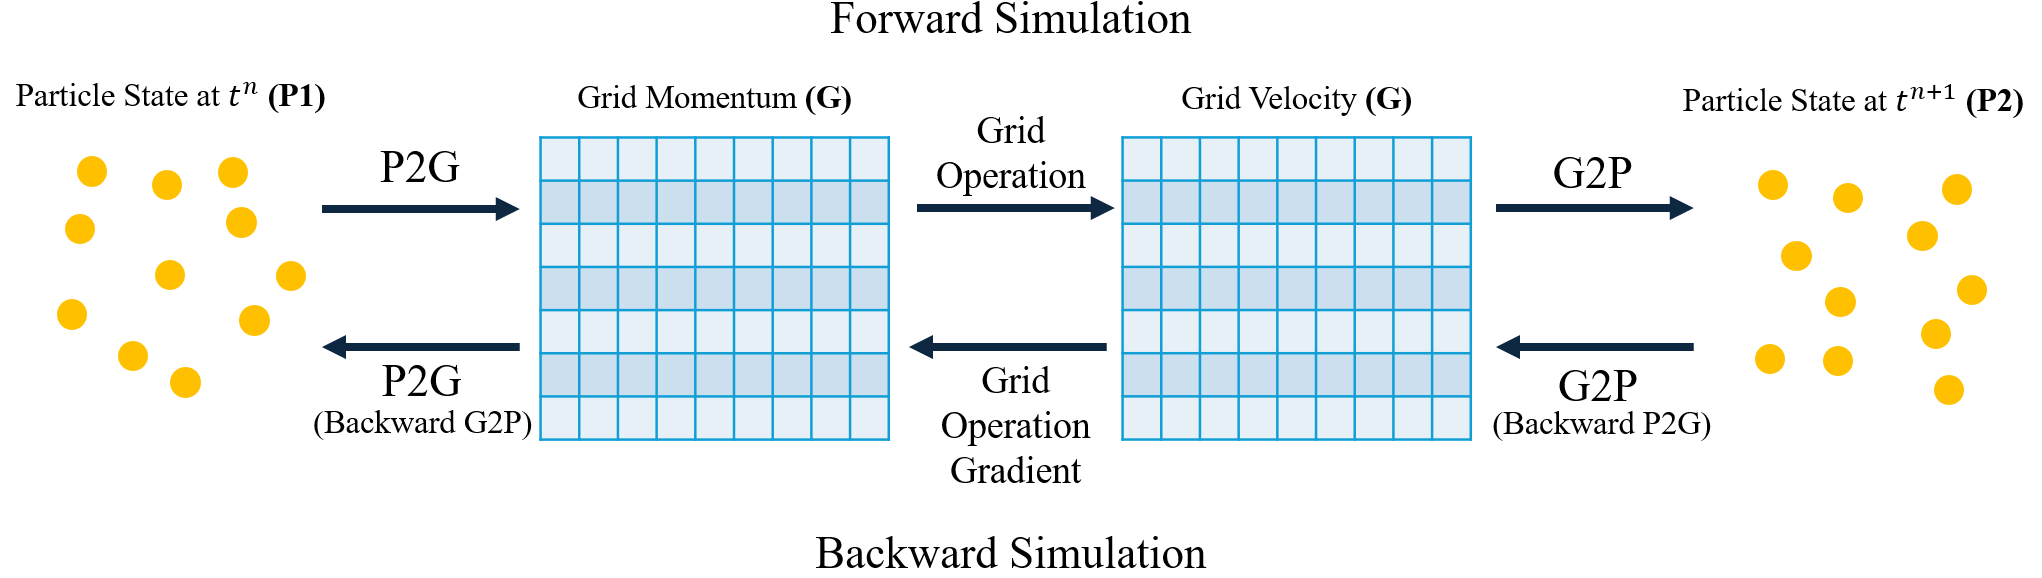
\includegraphics[width=\linewidth]{figs/MPM_MLS.png}
            \caption[{Simulation overview}]{\textbf{Simulation overview.} A timestep in {MPM} consists of five major computations: $\textbf{P1} \rightarrow \textbf{P2G} \rightarrow \textbf{G} \rightarrow \textbf{G2P} \rightarrow \textbf{P2}$. Particles store their own physical properties but interact with each other through the background simulation grid.}
            \label{fig:MLS_MPM}
        \end{figure*}
        
    The method starts with a continuum discretized into material points that carry physical properties of its domain, such as mass $m_p$, volume $V_p$, position $\mathbf{x}_p$, velocity $\mathbf{v}_p$, and deformation gradient $\mathbf{F}_p$.
    We use Affine Particle-in-Cell (APIC) transfer kernels \citep{jiang2017angular}, which further requires an affine matrix $\mathbf{C}_p$ to be stored on the particles.
    
    In MPM, updates to particle states are generally computed on a background grid.
    On each timestep, the background grid interpolates material point quantities like velocity to grid nodes, computes updates for quantities like momentum, then interpolates updated quantities back to the particles.
    The use of a regular background grid enables using efficient, scalable solvers that have been optimized for grids.
    
    Each timestep of the {MLS-MPM} algorithm we implement can be split into five major steps, as seen in Figure \ref{fig:MLS_MPM}:
        \begin{enumerate}
          \item \textbf{P1 (Particle Stress Calculation)}. For each particle, calculate its Piola-Kirchhoff stress tensor from its deformation gradient.
          \item \textbf{P2G (Particle to Grid)}. For each particle, interpolate its mass and momentum to the grid with APIC transfer kernels \citep{2015-APIC, jiang2017angular}.
          \item \textbf{G (Grid Velocity Calculation)}. For each grid node, solve for its updated momentum (incorporating any desired external forces) and velocities. % calculate its velocity from mass and momentum. Add any external force update to velocity here.
          Any time integration is performed using symplectic Euler.
          \item \textbf{G2P (Grid to Particle)}. For each particle, interpolate its updated velocity and affine matrix from the grid.
          \item \textbf{P2 (Particle Kinematic Update)}. For each particle, update its deformation gradient and position using the updated particle quantities and timestep.
        \end{enumerate}
    We refer the reader to \citet{2018-MLSMPM} and to the appendix for more detailed explanations of the {MLS-MPM} algorithm.

\subsection{Differentiable Simulation} 
    We implemented {MLS-MPM}, which is naturally differentiable; analytical gradients have been derived by \citet{2018-ChainQueen}. 
    We manually implemented the necessary analytical gradients to have more control over the implementation and avoid potential issues with software-based automatic differentiation \citep{johnson2023software}.
    In our method, these manually derived gradients were then used in conjunction with the non-stochastic version (i.e., all particles are used for each iteration) of the Adam optimizer \citep{kingma2014adam} to perform the optimization, ensuring stable and efficient convergence.
    In addition to optimization, a differentiable simulator naturally requires storing the feedforward simulation network to allow for the backpropagation of derivatives.
    We implemented this network by storing the computation graph of each timestep layer $\textbf{T}^n$, where a layer performs each step of an MPM timestep:

    \begin{equation}
        \textbf{T}^n = \textbf{P1}^n \rightarrow \textbf{P2G}^n \rightarrow \textbf{G}^n \rightarrow \textbf{G2P}^n \rightarrow \textbf{P2}^n .
    \end{equation}
    Backpropagation can then be used on the simulation network to compute gradients via the chain rule:
    \begin{equation}
        \textbf{T}^1 \leftarrow \cdots \leftarrow \textbf{T}^n \leftarrow \mathcal{L} .
    \end{equation}
    We refer to \citet{2018-ChainQueen} for the derivation of the analytical derivatives used in the backward pass. 
    Our method involves controlling particles' deformation gradients (Section \ref{sec:control}), so we introduce a control deformation gradient term separate from the time-evolved deformation gradients.
    The exact modification to the {MPM} algorithm can be seen in the appendix.
    These control deformation gradients are added in a way such that the loss gradient with respect to them is the same as the loss gradient with respect to the time-evolved deformation gradients.

\section{Deformation Gradient Control}
\label{sec:control}

    In continuum mechanics, an object has an initial domain in space
    denoted as $\Omega_0$. A point belonging to the object can be defined by its initial position $\textbf{X} \in \Omega_0$. As the object moves through space and time, the world coordinate of a point $\textbf{x}$ at some time $t$ can be represented as $\textbf{x} = \phi(\textbf{X}, t) \in \Omega_t$, where $\phi$ is known as a deformation map. The deformation gradient $\textbf{F}$ is defined as the Jacobian of the deformation map:
    \begin{equation}
        \mathbf{F}(\mathbf{X}, t) = \frac{\partial \phi}{\partial \mathbf{X}}(\mathbf{X}, t).
    \end{equation}
    
    It is common for elastic constitutive models to be defined on
    the deformation gradient $\textbf{F}$ such that internal energy is only built
    up when $\textbf{F}$ represents a non-rigid transformation between the rest
    state $\textbf{X}$ and the world state $\textbf{x}$. Our elastic energy function of choice is fixed corotated elasticity \citep{stomakhin2012energetically, jiang2016material}, whose Piola--Kirchhoff stress tensor is:
    \begin{equation}
        \textbf{P(F)} = 2\mu(\textbf{F - R}) + \lambda(J-1)J\textbf{F}^{-T},
    \end{equation}
    where $J$ is the determinant of $\mathbf{F}$ and $\mathbf{R}$ is its rotational component, which can be computed via the polar decomposition of $\mathbf{F}$ \citep{gast2016implicit}.
    
    Using this elastic model, we can manually control internal forces in our {MPM} simulation through the particle deformation gradients (we are inspired by the preliminary work of \citet{10.1145/3606037.3606840}).
    An example of this would be manually setting deformation gradients to the identity matrix $\mathbf{F} = \mathbf{I}$ after the shape has deformed. 
    This corresponds to setting the new rest state of the object to the current state. 
    Another way to control internal forces through deformation gradients would be setting expansion ($\alpha > 1$) and contraction ($\alpha < 1$) deformation gradients $\mathbf{F} = \alpha \mathbf{I}$.
    
    One might alternatively consider an approach that applies external forces to drive shape changes.
    However, if performing a shape morph using external forces, one needs to know precisely where to apply those forces on every timestep, and possibly extrinsic geometric surface properties like curvature; but as MPM represents objects with particles, it is not obvious where the surface of an object is at a given time step and what its local surface curvature is (especially when dealing with fine-scale/sub-grid geometric details).  Recent works have demonstrated the importance of and necessary care when dealing with MPM boundary representations and curvature, in simulating surface tension \citep{implicit_mpm_surface_tension,conservative_surface_tension}.    
    In contrast, directly optimizing the per-particle deformation gradient $\mathbf{F}$ eschews the modeling questions and numerical issues of dealing with external forces and takes advantage of the inherent properties of MPM.
    By focusing on $\mathbf{F}$ rather than external forces, we preserve physical consistency and achieve more stable, realistic morphing results in the context of MPM.
    
    Of course, to actually drive a shape morph, an automatic method for per-particle deformation gradient control is required.
    We achieve this through the optimization of the feedforward simulation network, which requires a loss function to be defined.

\subsection{Automatic Per-Particle Deformation Gradient Updates}
    \label{sec:control-updates}
    
    A key detail in our method is how the control deformation gradient $\tilde{\mathbf{F}}_p$ is optimized and accumulated into the particle deformation gradient $\mathbf{F}_p$ over time. 
    At each control timestep, we apply a direct update to $\tilde{\mathbf{F}}_p$ through gradient-based optimization, and accumulate it into $\mathbf{F}_p$. 
    The complete formulation is provided in Appendix~\ref{sec:appendixA}, which describes how the update is applied.
    This mechanism ensures that shape changes are persistent and physically consistent, rather than acting as temporary impulses. 
    To further improve stability and smoothness of the optimization, we apply a smoothing factor when updating $\tilde{\mathbf{F}}_p$.

\subsection{Preliminary Shape Loss Functions}
    To morph a shape from an input to a target geometry, we initially considered two simple loss function choices:

    \textit{Particle positions.} Given a simulation point cloud of size $N$, where
    each material point has a unique index $p \in [1, N]$, we require an
    equally sized target point cloud. A position-based loss function can then be defined as
    the sum of the squared distances between points $\mathbf{x}_p$ in the simulation
    point cloud and points $\mathbf{x}^*_p$ in the target point cloud:
    \begin{equation}
        \mathcal{L} = \sum_p \frac{1}{2}||\mathbf{x}_p - \mathbf{x}_p^*||^2 .
    \end{equation}
    In our experiments, this loss function is suitable for locomotion tasks or simple shape changes such as expansion or shearing;
    however, since it merely penalizes average position errors, using this loss function can leave outlier points in the morph and generally does not provide visually adequate morphs in the presence of fine-scale features or topology changes. 
    Another downside of using the position loss function is the requirement of an equally sized target point cloud with point-to-point correspondences.
    There are techniques available for computing the point-to-point correspondences of two different shapes \citep{2011-ShapeCorrespondenceSurvey}, but this places a constraint on the optimal positions of individual material points.

    \noindent \\ \textit{Nodal mass.}
    In {MPM}, we have the luxury of a background grid, whose nodes can store interpolated quantities such as mass from the particles.
    Using a nodal mass loss function instead of a point position loss function can alleviate many requirements on our input geometry, such as the need to have identical numbers of particles in the input and target geometries.
    
    We can then compute the sum of the squared differences between the nodal masses $m_i$ and $m_i^*$ of the interpolated input masses and the interpolated target masses, respectively:
    \begin{equation}
        \mathcal{L} = \sum_{i} \frac{1}{2} (m_i - m^*_i)^2 .
    \end{equation}
    
    This loss function is not easy to optimize with general optimizers and can result in ``mass ejections,'' where clumps of material points are violently propelled outward.
    Figure~\ref{fig:mass_ejection} illustrates such a scenario, where regions of the domain with large mass discrepancies cause particles to be ejected. 
    We believe that mass ejections are a consequence of converging to local minima of the nodal mass loss function, in which these ejections lead to the quickest decrease of the loss value.
    This problem becomes more noticeable with larger differences between the initial and target shapes.
    In such cases, a stronger force is applied in the parts of the domain with less overlap between input and target geometries (hence, a large difference in mass), resulting in even greater mass ejection.
    
    Knowing this, we designed a small modification to the nodal mass loss function to eliminate mass ejections.
    
    \begin{figure}[ht!]
        \centering
        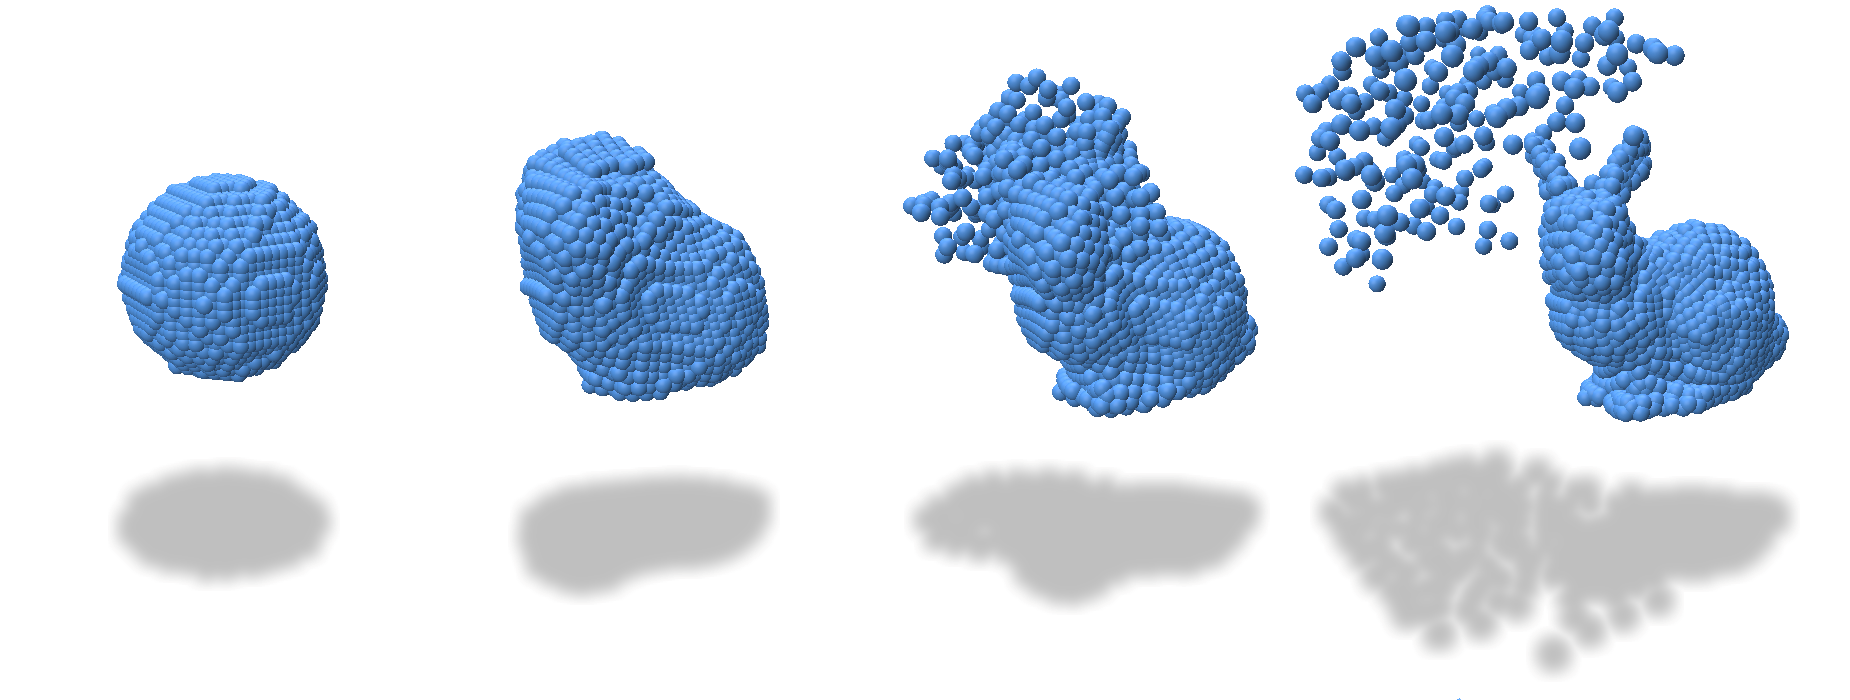
\includegraphics[width=\linewidth]{figs/mass_ejection.png}
        \caption[{An example of mass ejections occurring under the naive nodal mass loss}]{\textbf{An example of mass ejections occurring under the naive nodal mass loss.} Particles are forcefully ejected outward, leading to unstable or unrealistic behavior.}
        \label{fig:mass_ejection}
    \end{figure}

\subsection{Log-Based Mass Loss Function}  
    To address these limitations, we propose a novel loss formulation that simultaneously improves numerical stability and enforces physical plausibility.
    Specifically, we aim to construct a smoother loss landscape that is less sensitive to outliers and promotes stable optimization.
    To this end, we introduce a log-based mass loss function, defined as:
    
    \begin{equation}
        \mathcal{L} = \mathcal{L}_{\text{mass}} + \mathcal{L}_{\text{penalty}} ,
    \end{equation}
    \begin{equation}
        \mathcal{L}_{\text{mass}} = \sum_{i} \frac{1}{2} (\ln(m_i + 1 + \epsilon) - \ln(m^*_i + 1 + \epsilon))^2 ,
    \end{equation}
    \begin{equation}
        \mathcal{L}_{\text{penalty}} = \sum_{i} {1}_{\{m_i < m_{\text{min}}\}} \cdot w \cdot ( m_{\text{min}} - m_i )^2 .
    \end{equation}

    To ensure numerical stability during the log transformation, we add a small constant $\epsilon$ as well as 1 to the mass values. We use a fixed value of $\epsilon = 1 \times 10^{-4}$ throughout our experiments to ensure stable and consistent behavior.
    
    Additionally, to prevent physically implausible mass loss, we introduce a penalty term $\mathcal{L}_{\text{penalty}}$ for cases where the predicted mass $m_i$ falls below a predefined minimum threshold $m_{\text{min}}$. This penalty is scaled quadratically with the difference and weighted by a factor $w$, which we set to 10.0 in all our experiments. The magnitude of $w$ plays an important role in the optimization dynamics. Increasing $w$ makes the result closer to the target mesh but can introduce oscillations near the optimum. Conversely, decreasing $w$ reduces such oscillations but allows the result to deviate more from the target mesh.
    
    This loss function design allows us to mitigate the impact of outliers while softly constraining unrealistic mass depletion. As a result, we are able to effectively suppress mass ejection artifacts during simulation, as demonstrated in Section~\ref{sec:examples}.
    
      \begin{figure*}
            \centering
            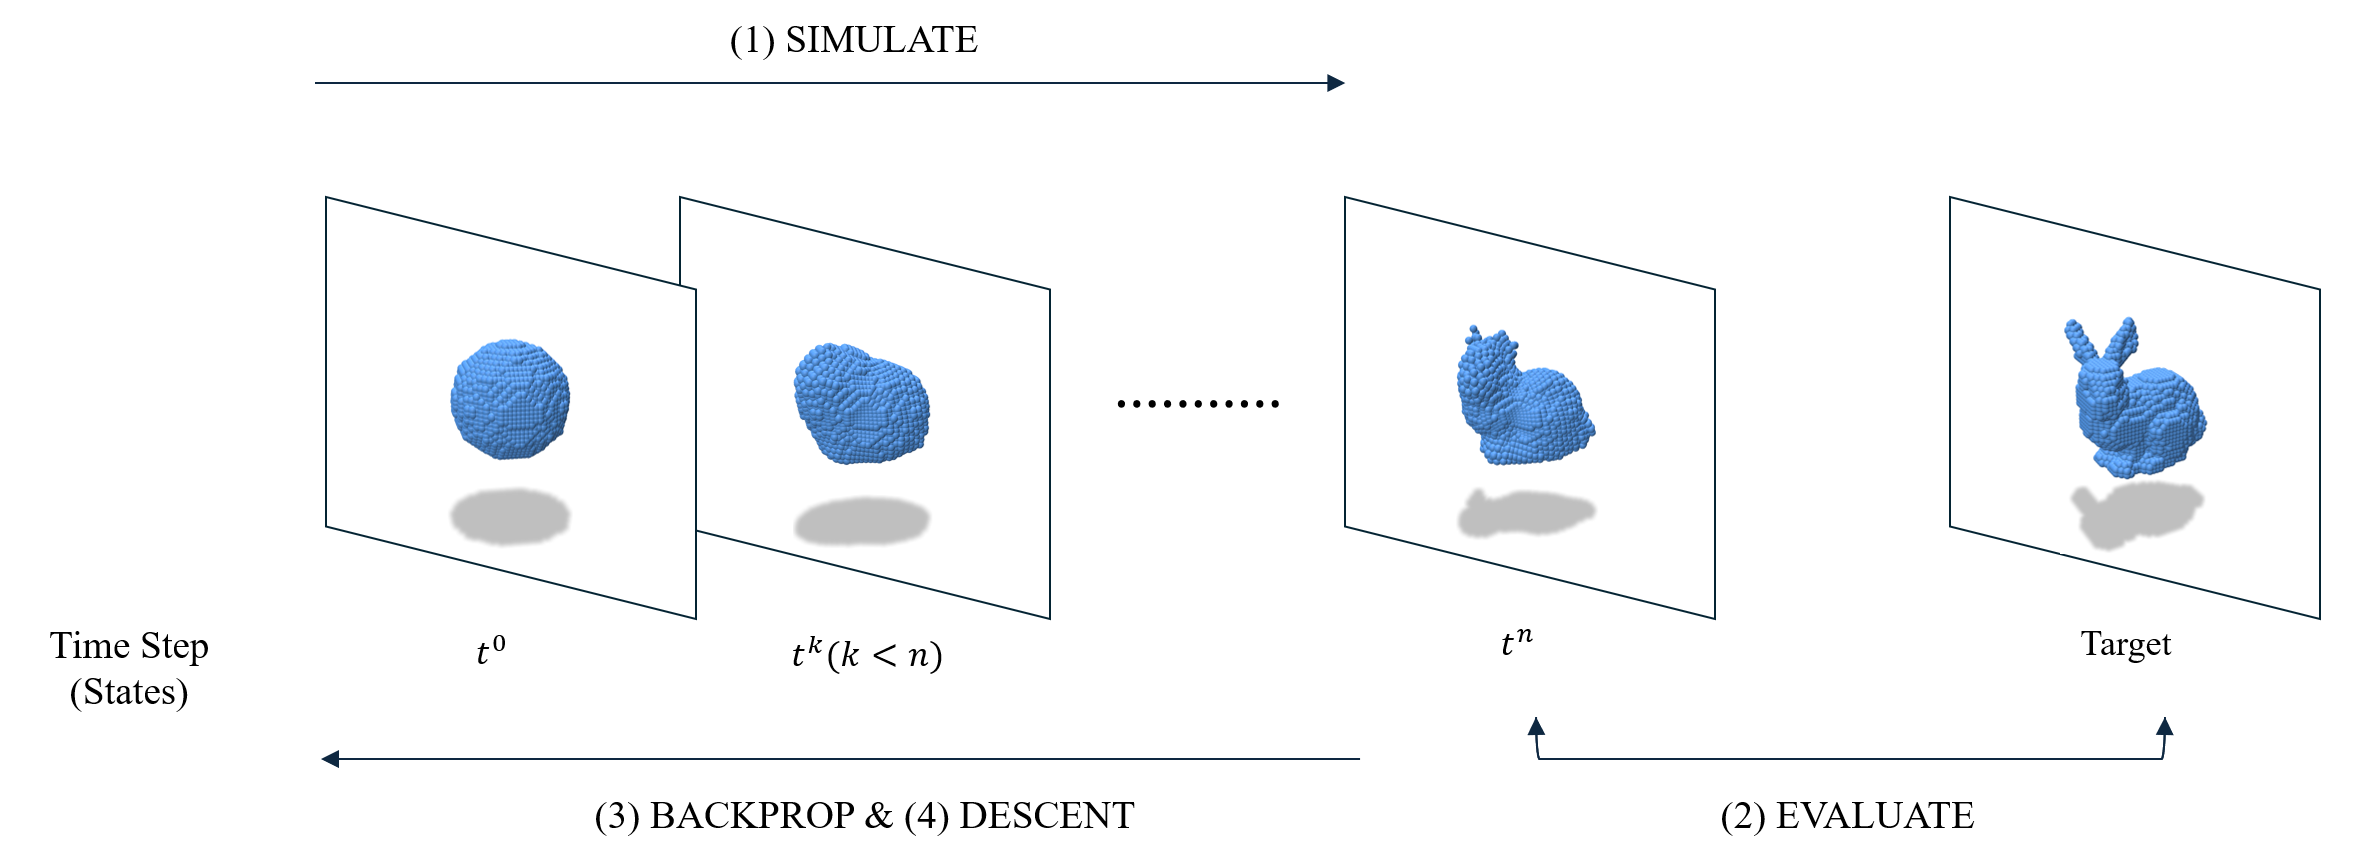
\includegraphics[width=\linewidth]{figs/fig_differ.png}
            \caption[{Morphing method}]{\textbf{Morphing method.} Step-by-step optimization process of the simulation networks, aligned according to the causality principle. The Adam optimizer for the control variables is implemented in order for each time step layer of the simulation and includes steps such as forward calculation ({SIMULATE}), loss function calculation ({EVALUATE}), backward calculation ({BACKPROP}), and control variable update ({DESCENT}). This optimization process can be repeated until the norm of the loss gradient falls below a certain tolerance.}
            \label{fig:Morphing}
        \end{figure*}
        
\section{Morphing Method}

    Given our simulation framework and loss function, we can now describe our proposed morphing algorithm. The main idea is based on Adam optimization of control deformation gradients.
    
\subsection{Simulation Optimization}
    In our simulation network in Figure \ref{fig:Morphing}, the ordering of operations is governed by the principle of causality. This means that any control or intervention applied at earlier stages has a direct impact on the inputs of subsequent layers, and consequently, on their outputs. In this context, ``control'' refers to any manipulation or condition imposed on the system, while ``layers'' represent the sequential stages of the simulation process.
    We outline the steps to perform an iteration of optimization on the control variables for a single timestep layer $\textbf{T}^n$ of the simulation network:
\begin{enumerate}
    \item \textbf{SIMULATE}. Compute the forward pass starting from the control layer to the final layer.
    \item \textbf{EVALUATE}. Compute the loss function via the final layer.
    \item \textbf{BACKPROP}. Compute the backward pass to get the gradient of the loss function with respect to the control variables in the control layer.
    \item \textbf{DESCENT}. Update the control variables by the loss function with Adam optimizer using the origin stepsize $\alpha$, which can be fixed or computed via line search. In our case, we use a bisection line search method (Algorithm \ref{alg:linesearch}) to find a step size that sufficiently decreases loss.
\end{enumerate}
    This process of optimization can be repeated until convergence, which can be defined as the norm of the loss gradient being below a specified tolerance. 
    Once the optimization for a single layer has been satisfactorily completed, the optimization can move on to the next layer.

\subsection{Control Layers}
\label{sec:control-layers}
    To save on computation time, and to allow time for the effects of previously controlled deformation gradients to propagate, we only compute control deformation gradients on a subset of the timesteps. 
    We denote the layers where we compute control deformation gradients as ``control layers.'' 
    Our simulation uses a timestep size of $\Delta t = 1/120$ seconds, and we apply control gradients every 10 timesteps.

    We outline in pseudocode our algorithm for computing the control deformation gradients using one optimization pass in Algorithm \ref{alg:mpm-morph}.
    To make the notation concise, we let $\tilde{\mathbf{F}}^n$ represent the control deformation gradients at timestep $n$.
    We also let Loss($\tilde{\mathbf{F}}^n$) represent forward simulation from timestep $n$ to $N$, followed by computing the loss between the material points at timestep $N$ and the target shape.
    We note that the partial derivative of the loss is first computed per grid node with respect to the nodal grid mass $m_i$, which will in general be distinct for different grid nodes. 
    Based on this quantity, we can then use MLS-MPM interpolatory weights to compute the derivative of loss with respect to a particle's location $\mathbf{x_p}$, and then apply the chain rule to compute derivatives of the loss with respect to per-particle control deformation gradients, the set of which is $\tilde{\mathbf{F}}^n$.
    The optimization step in Algorithm \ref{alg:mpm-morph} can then update each particle's control deformation gradient. We emphasize that with this algorithm, each particle will, in general, end up with distinct control deformation gradients.

   \begin{algorithm}
      \caption{Control Deformation Gradient Computation}\label{alg:mpm-morph}
      \begin{algorithmic}[1]
        \Require $N$, the final simulation timestep
        \Require $\Delta n$, the control period
        \Require $i_{\text{max}}$, the max number of iterations per control timestep
        \Require $\kappa$, the convergence tolerance for Adam optimizer
        \Require $\alpha$, the original Adam optimizer step size
        \Require $\beta_1$, $\beta_2$, the decay rates for the moment estimates
        \Require $\epsilon_{\text{adam}}$, a constant to avoid division by zero in Adam
    
        \State $\tilde{\mathbf{F}}^{1:N} \gets \mathbf{0}$ \Comment{Initialize control deformation gradients}
        \State $m^{1:N} \gets \mathbf{0}$ \Comment{First moment vector}
        \State $v^{1:N} \gets \mathbf{0}$ \Comment{Second moment vector}
        \State $t \gets 0$
        \State $n \gets 1$
    
        \While{$n < N$}
          \State $i \gets 0$
          \While{$i < i_{\text{max}}$}
            \State $L \gets \text{Loss}(\tilde{\mathbf{F}}^{n})$ \Comment{Loss after sim from $n$ to $N$}
            \State $\mathbf{g} \gets \dfrac{\partial L}{\partial \tilde{\mathbf{F}}^{n}}$ \Comment{Gradient}
    
            \State $m^{n} \gets \beta_1\, m^{n} + (1-\beta_1)\, \mathbf{g}$
            \State $v^{n} \gets \beta_2\, v^{n} + (1-\beta_2)\, (\mathbf{g} \odot \mathbf{g})$ \Comment{Hadamard product}
    
            \State $\hat{m}^{n} \gets \dfrac{m^{n}}{1-\beta_1^{t+1}}$ \Comment{Bias correction (use $t+1$ after update)}
            \State $\hat{v}^{n} \gets \dfrac{v^{n}}{1-\beta_2^{t+1}}$
    
            \State $\alpha \gets \text{ComputeStepSize}\big(L,\, \tilde{\mathbf{F}}^{n},\, \hat{m}^{n},\, \alpha\big)$
            \State $\tilde{\mathbf{F}}^{n} \gets \tilde{\mathbf{F}}^{n} - \alpha \dfrac{\hat{m}^{n}}{\sqrt{\hat{v}^{n}} + \epsilon_{\text{adam}}}$
    
            \If{$\lVert \mathbf{g} \rVert < \kappa$}
              \State \textbf{break}
            \EndIf
    
            \State $i \gets i + 1$
            \State $t \gets t + 1$
          \EndWhile
          \State $n \gets n + \Delta n$
        \EndWhile
    
        \State \Return $\tilde{\mathbf{F}}^{1:N}$
      \end{algorithmic}
    \end{algorithm}


    \begin{algorithm}
    \begin{algorithmic}[1]
        \Require $L_0$, the original loss
        \Require $\mathbf{x}$, the original vector argument
        \Require $\Delta \mathbf{x}$, the step direction vector
        \Require $\alpha$, the original step size
        \State $L \leftarrow $ Loss$(\mathbf{x} + \alpha \Delta \mathbf{x})$
        \While{$L > L_0$}
            \State $\alpha \leftarrow \alpha / 2$
            \State $L \leftarrow \text{Loss}(\mathbf{x} + \alpha \Delta \mathbf{x})$
        \EndWhile
        \State \textbf{return} $\alpha$ 
        \end{algorithmic}
    \caption{ComputeStepSize ($L_0$, $\mathbf{x}$, $\Delta \mathbf{x}$, $\alpha$)}\label{alg:linesearch}
    \end{algorithm}
    
\subsection{Multiple Optimization Passes}
    As described in the prior subsection, we use the routine of Algorithm \ref{alg:mpm-morph} to compute optimal control deformation gradients for each control layer.
    However, this strategy is suboptimal: for instance, when we compute optimal control deformation gradients for the first control layer, we are using values of 0 for the control deformation gradients at all subsequent control layers, when we know that we will later optimize those to also have non-zero values.
    Accordingly, to obtain improved control deformation gradient values, we can utilize a multi-pass optimization scheme where, after optimizing control deformation gradients at all control layers, we can go through and re-run the optimization routine of Algorithm \ref{alg:mpm-morph} using the computed $\tilde{\mathbf{F}}^{1:N}$ as initial/improved guesses for the optimization.
    
    For a clear analysis of the tradeoffs, we evaluated the impact of the number of passes and the number of gradient iterations on performance based on the data shown in Table \ref{tab:multipass}. This ablation study provides useful insights into the relationship between loss values and execution time. For example, there is a significant improvement in loss between 1 pass and 3 passes, while the execution time remains the same. This suggests that multi-pass optimization can improve the loss without degrading performance.

    Additionally, our analysis of the limitations of increasing the number of passes shows that beyond 6 or 12 passes, the loss values do not improve and may even increase. This indicates the limits of optimization, highlighting that a larger number of passes does not always guarantee better results.
    
    Lastly, we observed that despite varying the number of passes and gradient iterations, the execution time remains nearly constant. This is a significant finding, as it emphasizes that further optimization can reduce the loss without negatively impacting performance.
    
    \begin{table}[ht!]
        \centering
        \small
        \caption[{Varying the number of optimization passes and optimization iterations per pass}]{\textbf{Varying the number of optimization passes and optimization iterations per pass.}}
        \begin{tabular}{cccc}
        \toprule
        Passes & \# of Gradient Iter & Final Loss & Elapsed Time [s] \\
        \midrule
        1   & 12 & 92.3826 & 187 \\
        3   & 4  & 91.0895 & 187 \\
        6   & 2  & 93.4914 & 187 \\
        12  & 1  & 93.1483 & 186 \\
        \bottomrule
        \end{tabular}
        \label{tab:multipass}
    \end{table}
    
\subsection{Chaining Multiple Simulation Networks}
    The amount of memory required for a simulation network is directly proportional to the number of simulation timesteps.
    This can make long animations require an infeasible amount of memory.
    Furthermore, backpropagation through longer networks can result in accumulating floating point errors and in problems like vanishing gradients \citep{hochreiter1998vanishing}. 

    Therefore, for longer morph animations, we can divide the morph into different segments and optimize one segment at a time.
    We construct a new simulation network using the final layer of the previous optimized network.
    The animation produced by the previous network is saved to disk before the memory of the previous network is freed.
    The new network is then optimized, and this process repeats.
    In our experiments, we split the optimization for long animations into networks of 10 timesteps each, i.e., 0.083-second segments at 120 FPS.
    By chaining optimized simulation networks together, we can produce indefinitely longer animations without any increased memory requirements and with reduced computational cost.

   \begin{figure}[!ht]
        \centering
        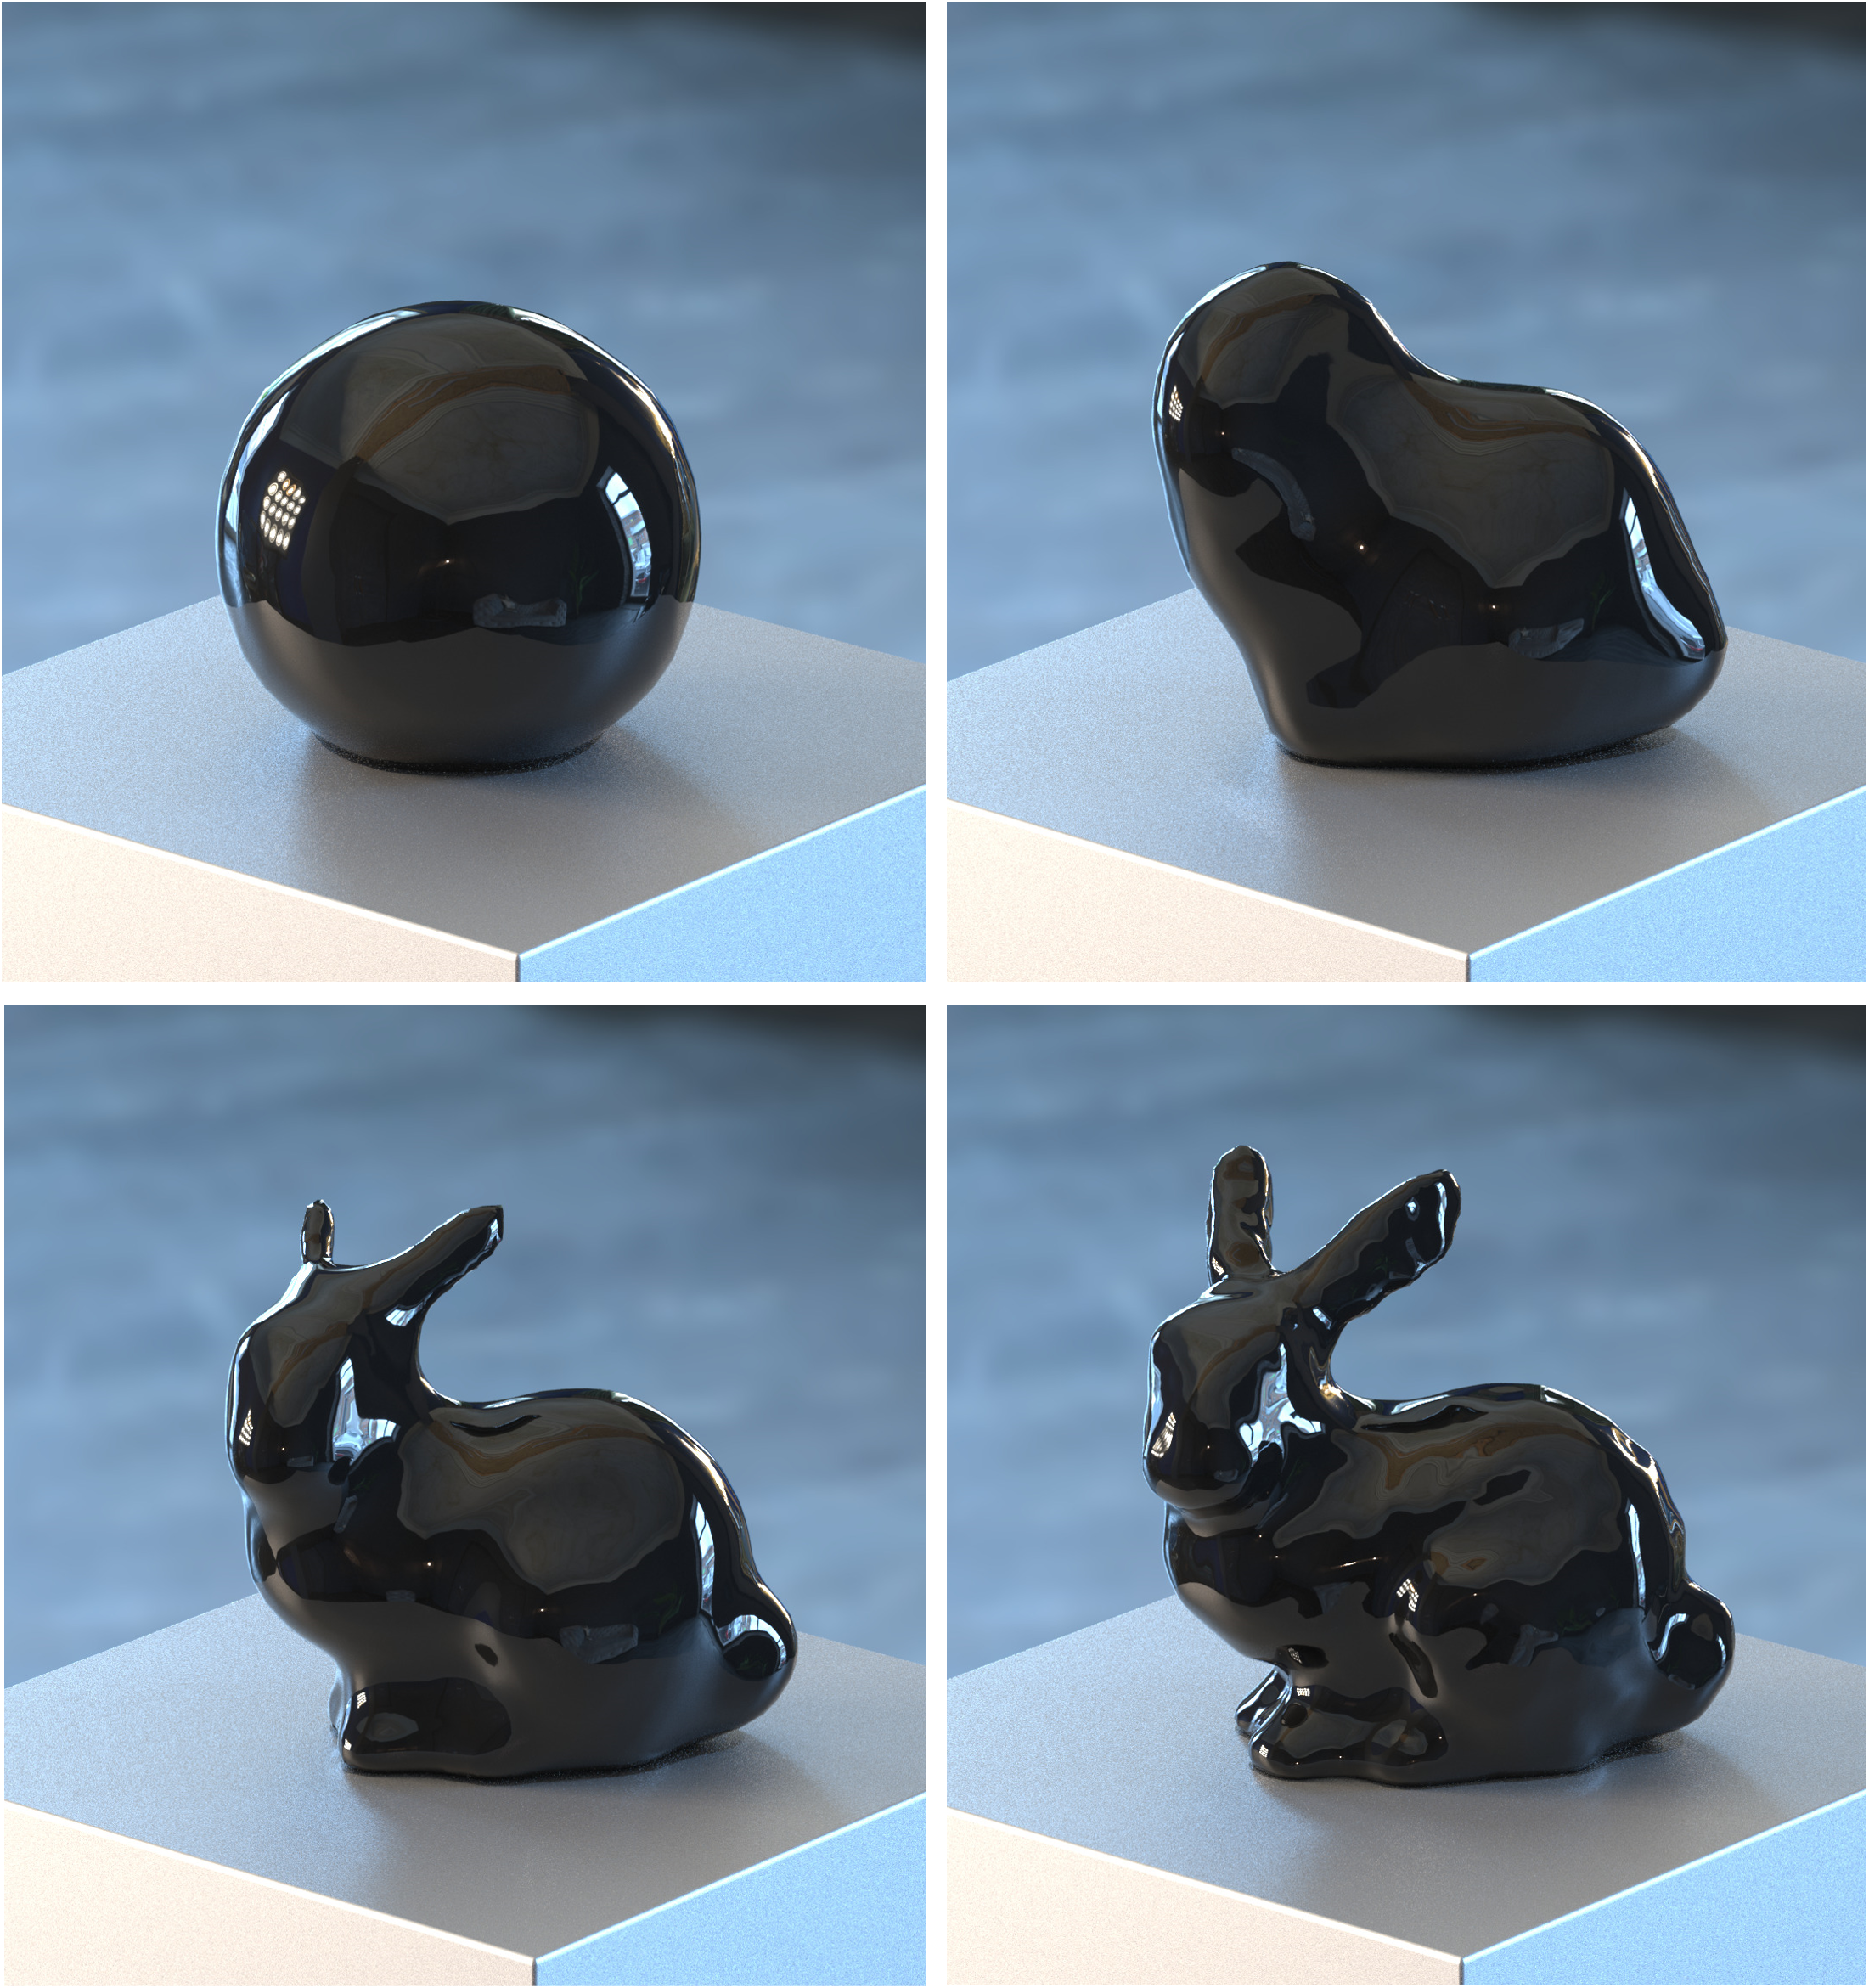
\includegraphics[width=\linewidth]{figs/Sphere_To_Bunny.png}
        \caption[{Sphere to bunny morphing animation}]{\textbf{Sphere to bunny morphing animation.} Key stages show the sphere evolving into a detailed bunny form, highlighting our method's precision in capturing sharp features like the ears.}
        \label{fig:Sphere@Bunny}
    \end{figure}

    \begin{figure}[!ht]
        \centering
        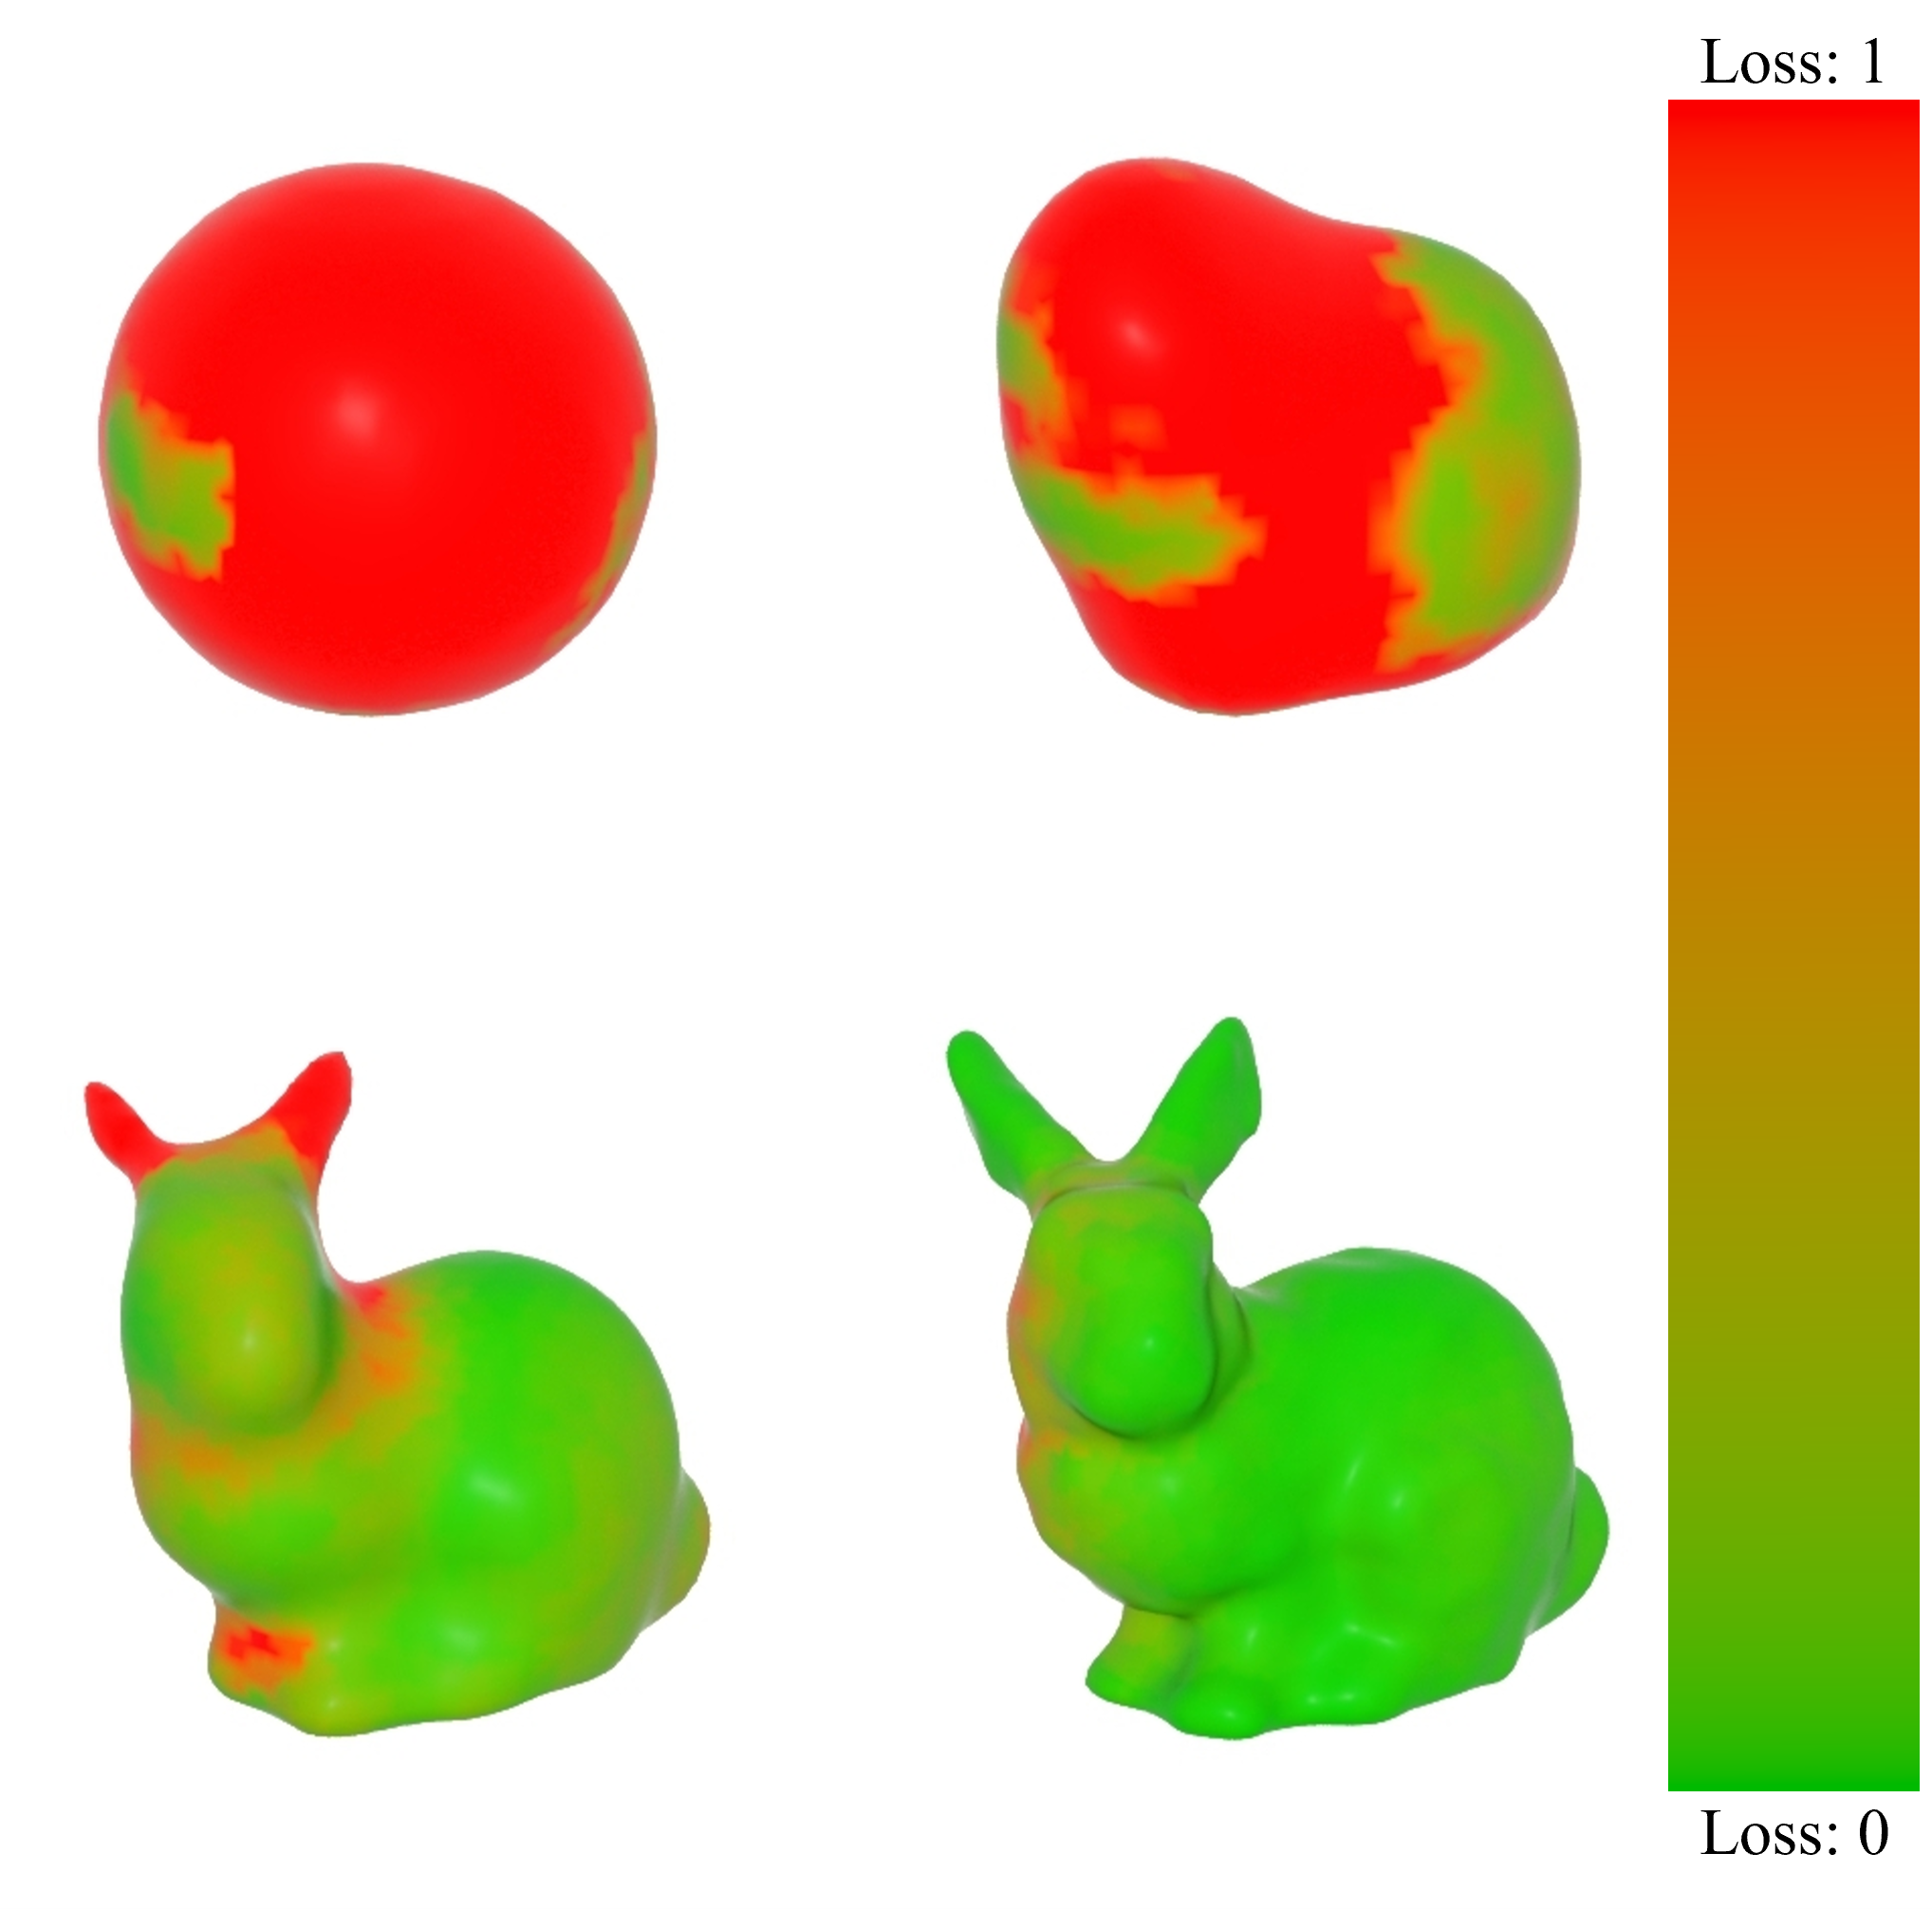
\includegraphics[width=\linewidth]{figs/Loss_visual.png}
        \caption[{Visualizing our loss function while morphing a sphere to a bunny}]{\textbf{Visualizing our loss function while morphing a sphere to a bunny.} Loss is normalized from 0 to 1 for ease of visualization. We observe a smooth decrease in the loss, including in the finer regions of the target geometry towards the end of the morph.} %\textmd{Depict initial and mid-transition stages with red areas indicating higher loss. The bottom shows the final bunny form with minimized loss, demonstrating the effectiveness of our Log-like mass loss function in stabilizing the morphing process.}}
        \label{fig:Loss}
    \end{figure}


\section{Examples}

% \begin{table*}[!ht]
%     \centering
%         \scriptsize
%         \caption{Parameters for the various pairwise morphing examples are summarized in Table~\ref{tab:params}. Density and smoothing factor $\gamma$ varied slightly between examples to improve the smoothness of the morph.}
%         \begin{tabularx}{1.0\textwidth}{@{}lcccccccc@{}}
%             \toprule
%             Example & \# of Frames & Density [kg/$m^3$] & $\gamma$ & dt &\# of Gradient Iter (\# of Path) & Target \# of Particles & Initial \# of Particles & Grid Resolution \\
%             \midrule
%             Sphere to Bunny	& 420 & 75 & 0.955 & 0.00833 & 4(3) & $1.116 \times 10^4 $ & $0.92 \times 10^4 $ & $32 \times 32 \times 32$ \\ % OK
%             Sphere to Bob   & 600 & 60 & 0.955 & 0.00833 & 4(3) & $1.116 \times 10^4 $ & $1.06 \times 10^4$ & $32 \times 32 \times 32$ 	\\ % OK
%             Sphere to Cow  & 400 & 60 & 0.955 & 0.00833 & 4(3) & $1.116 \times 10^4$ & $0.76 \times 10^4$ & $32 \times 32 \times 32$ 	\\ % OK
%             Sphere to Car   & 450  & 60 & 0.955  & 0.00833 & 4(3) & $1.116 \times 10^4$ & $1.21 \times 10^4$ & $32 \times 32 \times 32$ 	\\ % OK
            
%             \midrule
%             Bob to Sphere   & 450 & 70 & 0.950 & 0.00833 & 4(3) & $1.06 \times 10^4$ & $1.11 \times 10^4$ & $32 \times 32 \times 32$ 	  \\ % OK 
%             Bob to Bunny    & 600 & 75 & 0.955 & 0.00833 & 4(3) & $1.06 \times 10^4$ & $0.92 \times 10^4 $ & $32 \times 32 \times 32$       \\ % OK  
%             Bob to Cow	    & 500 & 75	& 0.955  & 0.00833 & 4(3) & $1.06 \times 10^4$ & $0.76 \times 10^4$ & $32 \times 32 \times 32$ 	    \\ % OK
%             Bob to Car	    & 600 & 60	& 0.940  & 0.00833 & 4(3) & $1.06 \times 10^4$ & $1.06 \times 10^4$ & $32 \times 32 \times 32$ 	    \\ % OK
            
%             \midrule
%             Bunny to Sphere	& 500 & 100 & 0.965 & 0.00833 & 4(3) & $0.92 \times 10^4 $ & $1.116 \times 10^4$ & $32 \times 32 \times 32$    \\ % OK
%             Bunny to Bob	& 630 & 120 & 0.96 & 0.00833 & 4(3) & $0.92 \times 10^4 $ & $1.116 \times 10^4$ & $32 \times 32 \times 32$ 	\\ % OK
%             Bunny to Cow	& 400 & 110 & 0.955 & 0.00833 & 4(3) & $0.92 \times 10^4 $ & $0.76 \times 10^4 $ & $32 \times 32 \times 32$ \\ % OK
%             Bunny to Car	& 850 & 75 & 0.955 & 0.00833 & 4(3) & $0.92 \times 10^4 $ & $1.21 \times 10^4$ & $32 \times 32 \times 32$ 	\\ % OK
            
%             \midrule			
%             Cow to Sphere	& 400	& 75 & 0.955 & 0.00833 & 4(3) & $0.76 \times 10^4$ & $1.116 \times 10^4$ & $32 \times 32 \times 32$  \\ % OK
%             Cow to Bunny	& 400	& 75 & 0.955 & 0.00833 & 4(3) & $0.76 \times 10^4$ & $0.92 \times 10^4 $ & $32 \times 32 \times 32$  \\ % OK
%             Cow to Bob	    & 600	& 75 & 0.955 & 0.00833 & 4(3) & $0.76 \times 10^4$ & $1.06 \times 10^4$ & $32 \times 32 \times 32$ 	 \\ % OK
%             Cow to Car	    & 600	& 75 & 0.955 & 0.00833 & 4(3) & $0.76 \times 10^4$ & $1.21 \times 10^4$ & $32 \times 32 \times 32$ 	 \\ % OK
%             \midrule			
%             Car to Sphere	& 600   & 75 & 0.950  & 0.00833 & 4(3) & $1.21 \times 10^4$ & $1.116 \times 10^4$ & $32 \times 32 \times 32$      \\ % OK 
%             Car to Bunny	& 600	& 75 & 0.930  & 0.00833 & 4(3) & $1.21 \times 10^4$ & $0.92 \times 10^4$ & $32 \times 32 \times 32$  	\\ % OK
%             Car to Bob	    & 300	& 60 & 0.955  & 0.00833 & 4(3) & $1.21 \times 10^4$ & $1.06 \times 10^4$ & $32 \times 32 \times 32$    \\ 
%             Car to Cow	    & 600	& 75 & 0.955 & 0.00833 & 4(3) & $1.21 \times 10^4$ & $0.76 \times 10^4$ & $32 \times 32 \times 32$   \\ % OK
%             \bottomrule
%         \end{tabularx}
%     \vspace{1mm}
%     \label{tab:params}
% \end{table*}

\begin{table*}[!ht]
\centering
\scriptsize
\caption[{All example pairs used in our morphing experiments}]{\textbf{All example pairs used in our morphing experiments are listed below.} We report the number of simulation steps (time steps), particle density, smoothing factor $\gamma$, and the number of particles for both the initial and target meshes. 
    For all examples, we used a fixed timestep size $\Delta t = 1/120$\,s, performed 4 gradient descent iterations (3 optimization passes), and employed a $32^3$ simulation grid. 
    \textit{Note:} Due to the small timestep size selected for high-resolution visualization, the resulting simulations effectively represent slow-motion morphing sequences.}

\begin{tabular}{l c c c c c c}
    \toprule
    \textbf{Start Mesh} & \textbf{End Mesh} & \textbf{\# of Timesteps} & \textbf{Density} & \textbf{Smoothing factor} \boldmath$\gamma$ & \textbf{Target \# of Particles} & \textbf{Initial \# of Particles} \\
    \midrule
    \multirow{4}{*}{Sphere}
      & Bunny & 420 & 75 & 0.955 & $1.116 \times 10^4$ & $0.92 \times 10^4$ \\
      & Bob   & 600 & 60 & 0.955 & $1.116 \times 10^4$ & $1.06 \times 10^4$ \\
      & Cow  & 400 & 60 & 0.955 & $1.116 \times 10^4$ & $0.76 \times 10^4$ \\
      & Car   & 450 & 60 & 0.955 & $1.116 \times 10^4$ & $1.21 \times 10^4$ \\
    \midrule
    \multirow{4}{*}{Bob}
      & Sphere & 450 & 70 & 0.950 & $1.06 \times 10^4$ & $1.11 \times 10^4$ \\
      & Bunny  & 600 & 75 & 0.955 & $1.06 \times 10^4$ & $0.92 \times 10^4$ \\
      & Cow   & 500 & 75 & 0.955 & $1.06 \times 10^4$ & $0.76 \times 10^4$ \\
      & Car    & 600 & 60 & 0.940 & $1.06 \times 10^4$ & $1.06 \times 10^4$ \\
    \midrule
    \multirow{4}{*}{Bunny}
      & Sphere & 500 & 100 & 0.965 & $0.92 \times 10^4$  & $1.116 \times 10^4$ \\
      & Bob    & 630 & 120 & 0.96  & $0.92 \times 10^4$  & $1.116 \times 10^4$ \\
      & Cow   & 400 & 110 & 0.955 & $0.92 \times 10^4$  & $0.76 \times 10^4$ \\
      & Car    & 850 & 75  & 0.955 & $0.92 \times 10^4$  & $1.21 \times 10^4$ \\
    \midrule
    \multirow{4}{*}{Cow}
      & Sphere & 400 & 75 & 0.955 & $0.76 \times 10^4$ & $1.116 \times 10^4$ \\
      & Bunny  & 400 & 75 & 0.955 & $0.76 \times 10^4$ & $0.92 \times 10^4$ \\
      & Bob    & 600 & 75 & 0.955 & $0.76 \times 10^4$ & $1.06 \times 10^4$ \\
      & Car    & 600 & 75 & 0.955 & $0.76 \times 10^4$ & $1.21 \times 10^4$ \\
    \midrule
    \multirow{4}{*}{Car}
      & Sphere & 600 & 75 & 0.950 & $1.21 \times 10^4$ & $1.116 \times 10^4$ \\
      & Bunny  & 600 & 75 & 0.930 & $1.21 \times 10^4$ & $0.92 \times 10^4$ \\
      & Bob    & 300 & 60 & 0.955 & $1.21 \times 10^4$ & $1.06 \times 10^4$ \\
      & Cow   & 600 & 75 & 0.955 & $1.21 \times 10^4$ & $0.76 \times 10^4$ \\
    \bottomrule
    \end{tabular}
    \label{tab:params}
\end{table*}




\label{sec:examples}

    We demonstrate our methodology on a wide range of physically-based morphing animations in three-dimensional space.
    Leveraging MPM, our objects can seamlessly undergo topological morphs driven by internal elastic forces.
    We use a modified explicit time integration scheme for {MLS-MPM} (see the appendix), which helps prevent instability when taking larger timesteps.
    %To mitigate these issues, we have modified the explicit MPM approach, which we thoroughly explain in the appendix of this paper.
    A full list of variables involved in our {MPM} implementation is also found in the appendix. % (Table \ref{tab:mpm-syms}).
    %Furthermore, we have introduced symbolic representations for generating morphing animations, which are detailed in Table \ref{tab:mpm-syms}
    
    % Parameters for all our experiments are summarized in Table \ref{tab:params}.
    %Deformation convergence tolerance was uniformly set to $0.001$ across all test cases.
    % {MPM} point cloud visualization was performed using Polyscope \citep{polyscope}, and rendering was conducted using Houdini.

    The pairwise morphing results across five distinct meshes are shown in Figure~\ref{fig:Overall_deform}, and the corresponding experimental parameters are summarized in Table~\ref{tab:params}.
    The table lists the number of particles in both the initial and target meshes.
    While the number of particles does not change during the morphing process---the particle count used for each animation is fixed to the number of particles in the initial mesh---the number of particles in the target mesh can also affect performance (so we report this number as well).
    This is because the target mesh particles are used in computations of the various derivatives of the loss function used during the backpropagation step of our algorithm.
    For all our examples, MPM point cloud visualization was performed using Polyscope \citep{polyscope}, and rendering was conducted using Houdini.
    We ran all experiments on a machine with an Intel i9-13950HX CPU, 32GB RAM, and an NVIDIA RTX 4090 GPU.

    \textit{Sphere to Bunny.} In our first example,  we present a morphing animation from a sphere to a bunny, as depicted in Figure \ref{fig:Sphere@Bunny}. This demonstrates a successful shape morph using our log-based nodal mass loss function (see supplemental video). While using other loss functions might result in phenomena like mass ejection, our method, as shown in the figure, allows for smooth transformation without ejected particles or other unpleasant artifacts.
    
    One of the most notable aspects of this example is the representation of the bunny's ears.
    Our methodology allows us not only to match the bulk volume of a target mesh but also to faithfully reproduce its sharp and thin features.
    %In contrast, conventional {MPM} techniques struggle to express such features due to the inherent dissipation of physical values during particle-grid transfers.
    %Using our chosen {MLS-MPM} approach proved to be important for accurately preserving geometric details like these.



    We also plot the loss function, interpolated to the surface, as the geometry deforms; see Figure \ref{fig:Loss}.
    The loss function is normalized from 0 to 1 in this figure for ease of visualization.
    We observe that the loss function smoothly decreases as the morph proceeds, with fine-scale details of the target mesh generally being the last parts of the morph to reach an acceptable state. % (below our deformation gradient convergence threshold).
    
    \textit{Duck (Bob) to Cow.} In the second example, we illustrate an animation transitioning from a duck model (``Bob'') to a cow model (``Cow'') in Figure \ref{fig:Duck@Cow}.
    This case is interesting due to the changing topology between the two geometries.
    %as the inflatable duc significant as it examines the ability of our approach to maintain stability even in the presence of a central hole in the mesh.
    Our method achieves a smooth morph of the geometry and topology simultaneously, which is a natural benefit of our underlying {MPM} framework. %The outcome demonstrates a seamless transformation into a cow, with the hole smoothly closing, as depicted in the figure. This example underscores the versatility of our methodology in representing not only partially perforated meshes but also meshes with complex concave or convex structures.

     \begin{figure}
        \centering
        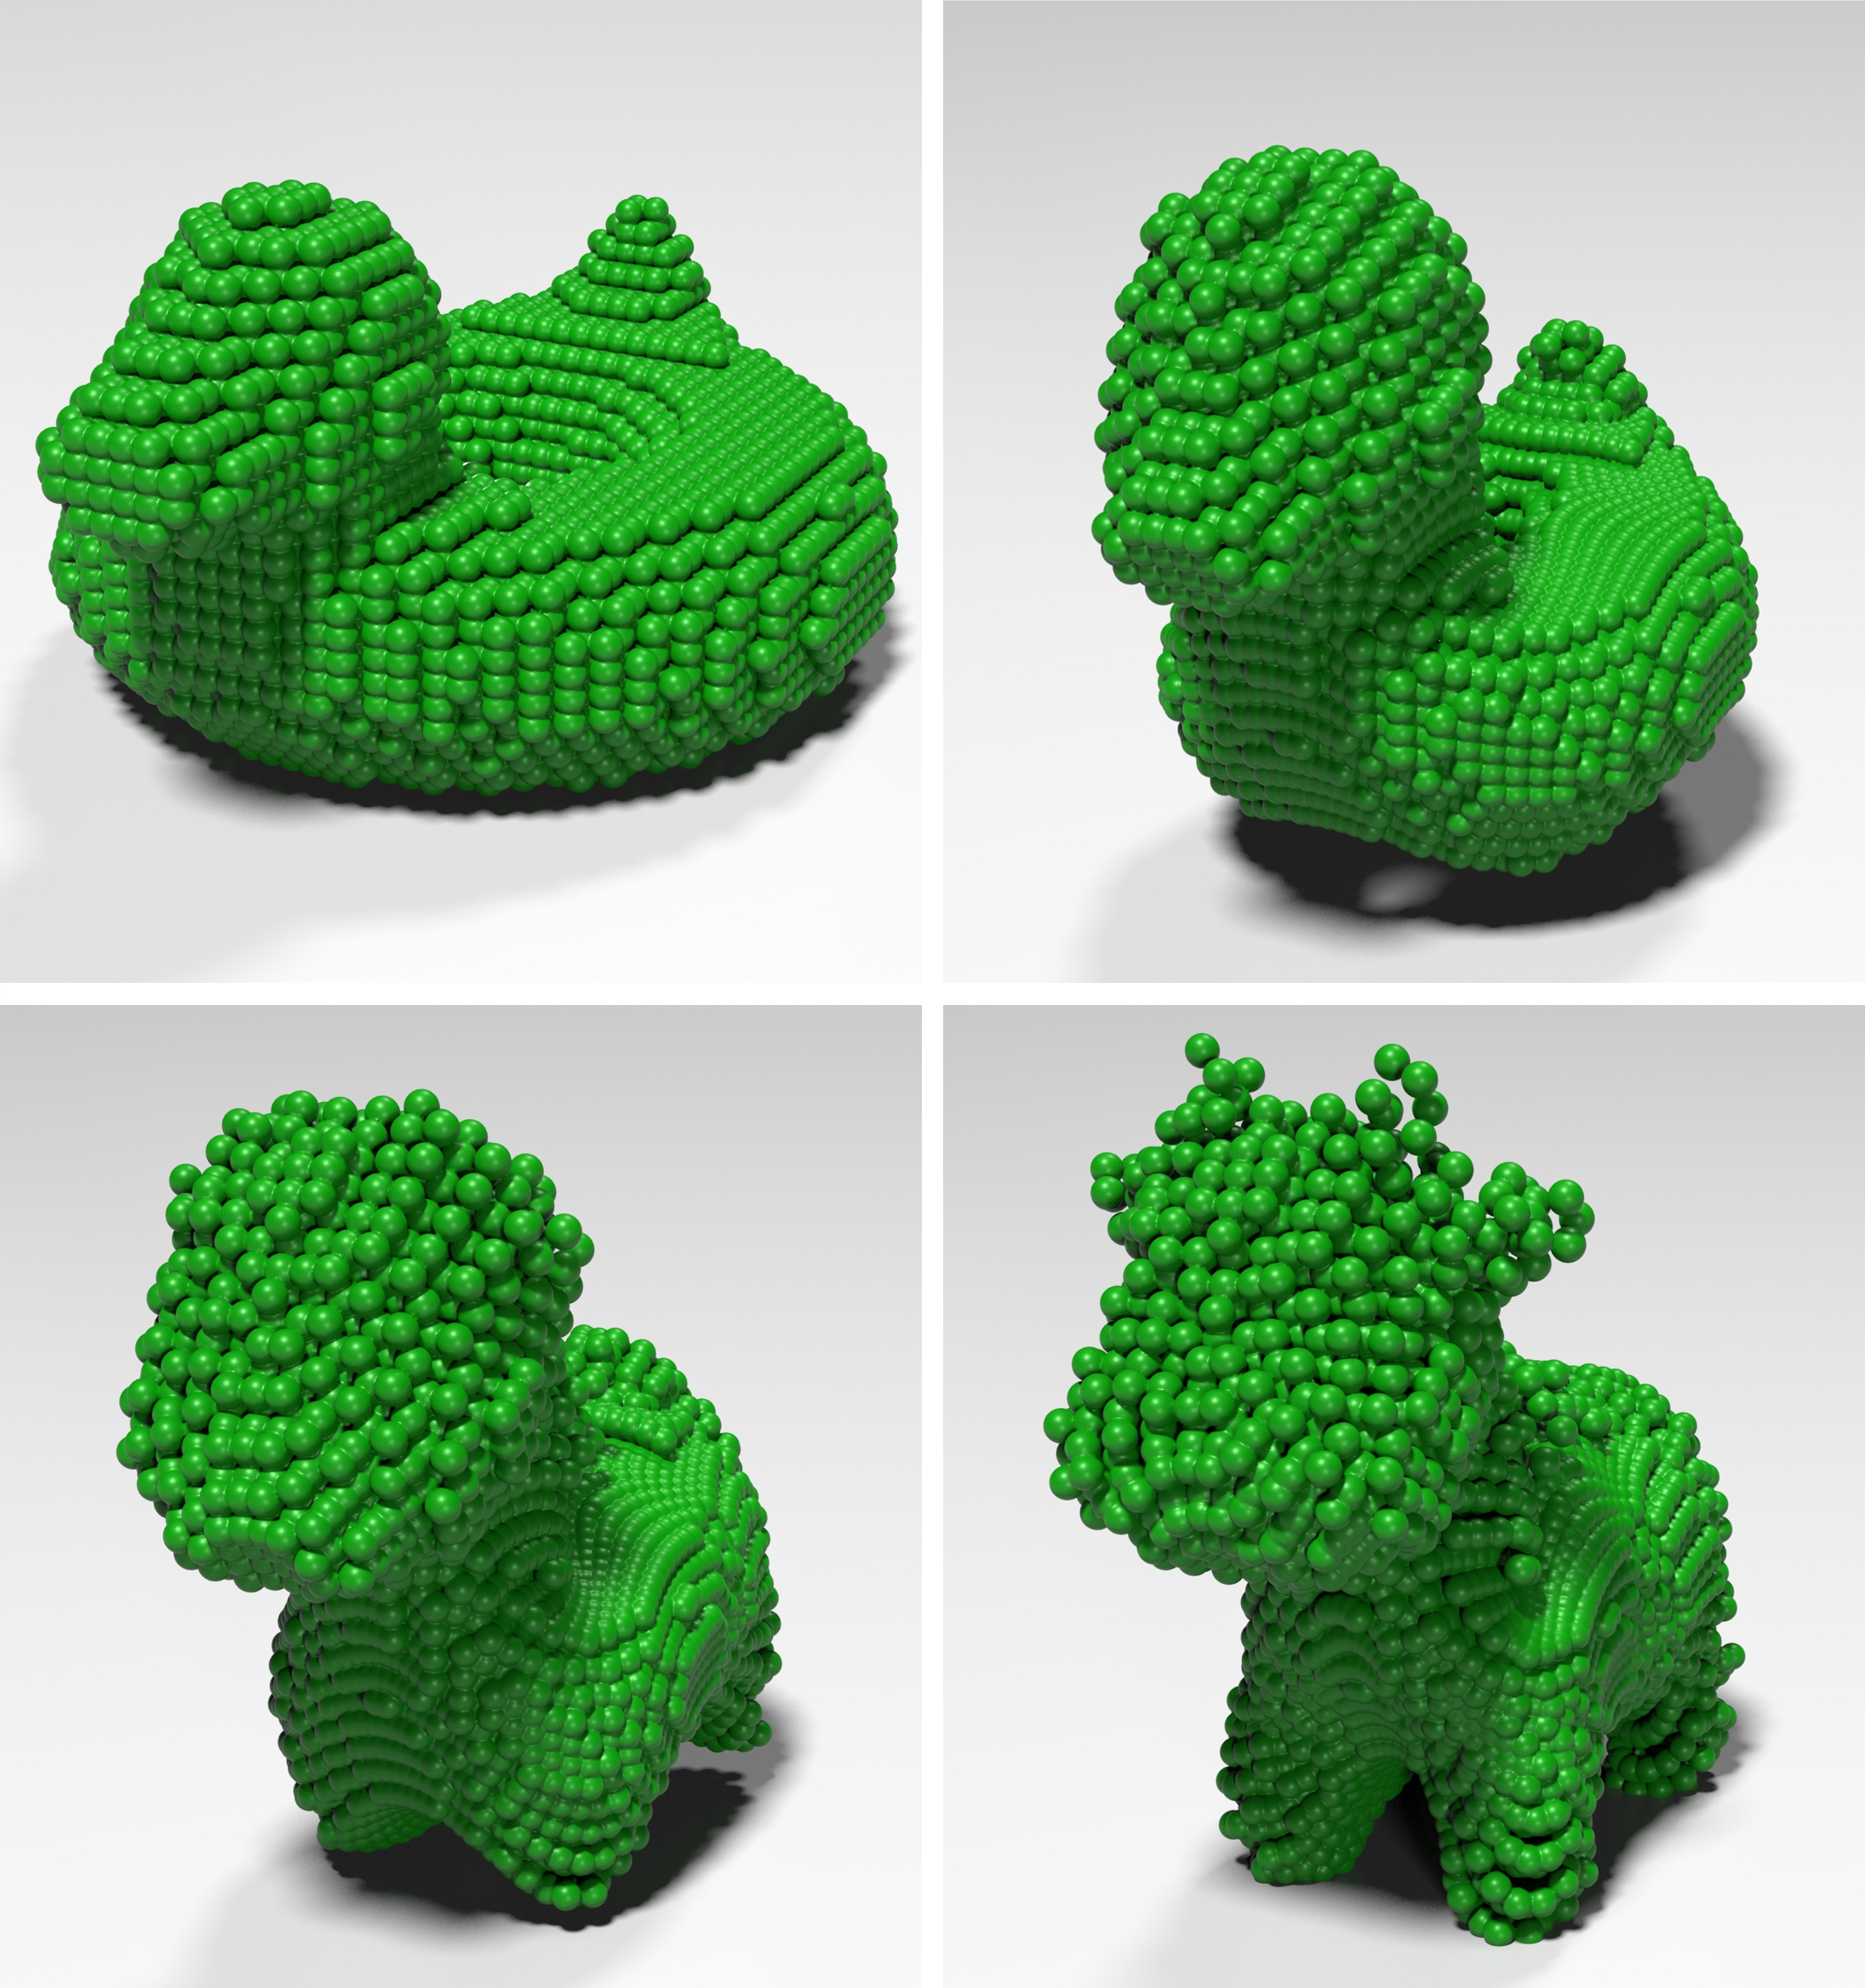
\includegraphics[width=\linewidth]{figs/Bob_To_Spot.png}
        \caption[{Morphing Duck (Bob) to Cow}]{\textbf{Morphing Duck (Bob) to Cow.} As the model deforms into a cow, we observe a smooth topology change as the center hole of the inflatable duck closes. This example evidences our method's ability to handle simultaneously evolving geometry and topology.}
        \label{fig:Duck@Cow}
    \end{figure}
    
\begin{table}[ht!]
  \scriptsize
  \caption[{Performance for various shape morphing sequences}]{\textbf{Performance for various shape morphing sequences, including accuracy (Final Loss is bolded for emphasis).}}
  \centering
  \begin{tabular}{llccc}
    \toprule
    \textbf{Start Mesh} & \textbf{End Mesh} 
    & \textbf{Time [s]} & \textbf{Loss (Initial $\rightarrow$ \textbf{Final})} & \textbf{Acc [\%]} \\
    \midrule
    \multirow{4}{*}{Sphere}
      & Bunny & 187 & 5302.69 $\rightarrow$ \textbf{91.09} & 98.28 \\
      & Cow  & 172 & 7685.97 $\rightarrow$ \textbf{124.43} & 98.38 \\
      & Car   & 188 & 8163.73 $\rightarrow$ \textbf{104.36} & 98.72 \\
      & Bob   & 290 & 11600.0 $\rightarrow$ \textbf{300.53} & 97.41 \\
    \midrule
    \multirow{4}{*}{Bob}
      & Sphere & 173 & 12018.7 $\rightarrow$ \textbf{388.20} & 96.77 \\
      & Bunny  & 332 & 12055.2 $\rightarrow$ \textbf{166.26} & 98.62 \\
      & Cow   & 195 & 12218.3 $\rightarrow$ \textbf{206.33} & 98.31 \\
      & Car    & 266 & 11516.7 $\rightarrow$ \textbf{368.94} & 96.80 \\
    \midrule
    \multirow{4}{*}{Bunny}
      & Sphere & 223 & 6104.12 $\rightarrow$ \textbf{119.75} & 98.04 \\
      & Bob    & 278 & 14184.2 $\rightarrow$ \textbf{608.07} & 95.71 \\
      & Cow   & 165 & 4469.88 $\rightarrow$ \textbf{70.51} & 98.42 \\
      & Car    & 415 & 11945.2 $\rightarrow$ \textbf{870.81} & 92.71 \\
    \midrule
    \multirow{4}{*}{Cow}
      & Sphere & 123 & 8606.47 $\rightarrow$ \textbf{465.71} & 94.59 \\
      & Bunny  & 120 & 3694.31 $\rightarrow$ \textbf{116.35} & 96.85 \\
      & Bob    & 178 & 12218.3 $\rightarrow$ \textbf{575.58} & 95.29 \\
      & Car    & 204 & 14316.9 $\rightarrow$ \textbf{685.36} & 95.21 \\
    \midrule
    \multirow{4}{*}{Car}
      & Sphere & 333 & 9980.66 $\rightarrow$ \textbf{122.11} & 98.78 \\
      & Bunny  & 335 & 11945.2 $\rightarrow$ \textbf{108.53} & 99.09 \\
      & Bob    & 309 & 11516.7 $\rightarrow$ \textbf{398.10} & 96.54 \\
      & Cow   & 333 & 14316.9 $\rightarrow$ \textbf{167.97} & 98.83 \\
    \bottomrule
  \end{tabular}
  \label{tab:performance}
\end{table}





    % \textit{Morphing between various mesh pairs; smoothing factor.} To further test our method, we explored pairwise deformations across a diverse set of five distinct meshes; see Table~\ref{tab:params}.
    % We aimed to rigorously assess the efficacy and reliability of our computational framework under varying geometric conditions.
    % All attempted morphs were successful, demonstrating the robustness and adaptability of our approach.
    % An additional element in achieving such a high degree of success was the interpolation of a deformation gradient mechanism ($\textbf{F}^{n+1} = (1 - \gamma)\textbf{F}^{n+1} + \gamma\textbf{F}^{n}$) during the post-processing phase. 
    
    % The smoothness values $\gamma$ we chose are reported in Table \ref{tab:params}, and were hand-tuned per example (generally keeping them as small as possible, while ensuring a smooth morphing animation).

    \textit{Morphing Between Various Mesh Pairs.}
    \label{sec:morphing-smoothing}
    To further test our method, we explored pairwise deformations across five distinct meshes (Figure~\ref{fig:Overall_deform}) under varying geometric conditions, with the experimental configurations summarized in Table~\ref{tab:params}.
    All attempted morphs were successful, demonstrating the robustness and adaptability of our approach.
    We also explored how varying smoothing factors and optimization algorithms affected the results:

    \begin{figure}[!htbp]
        \centering
        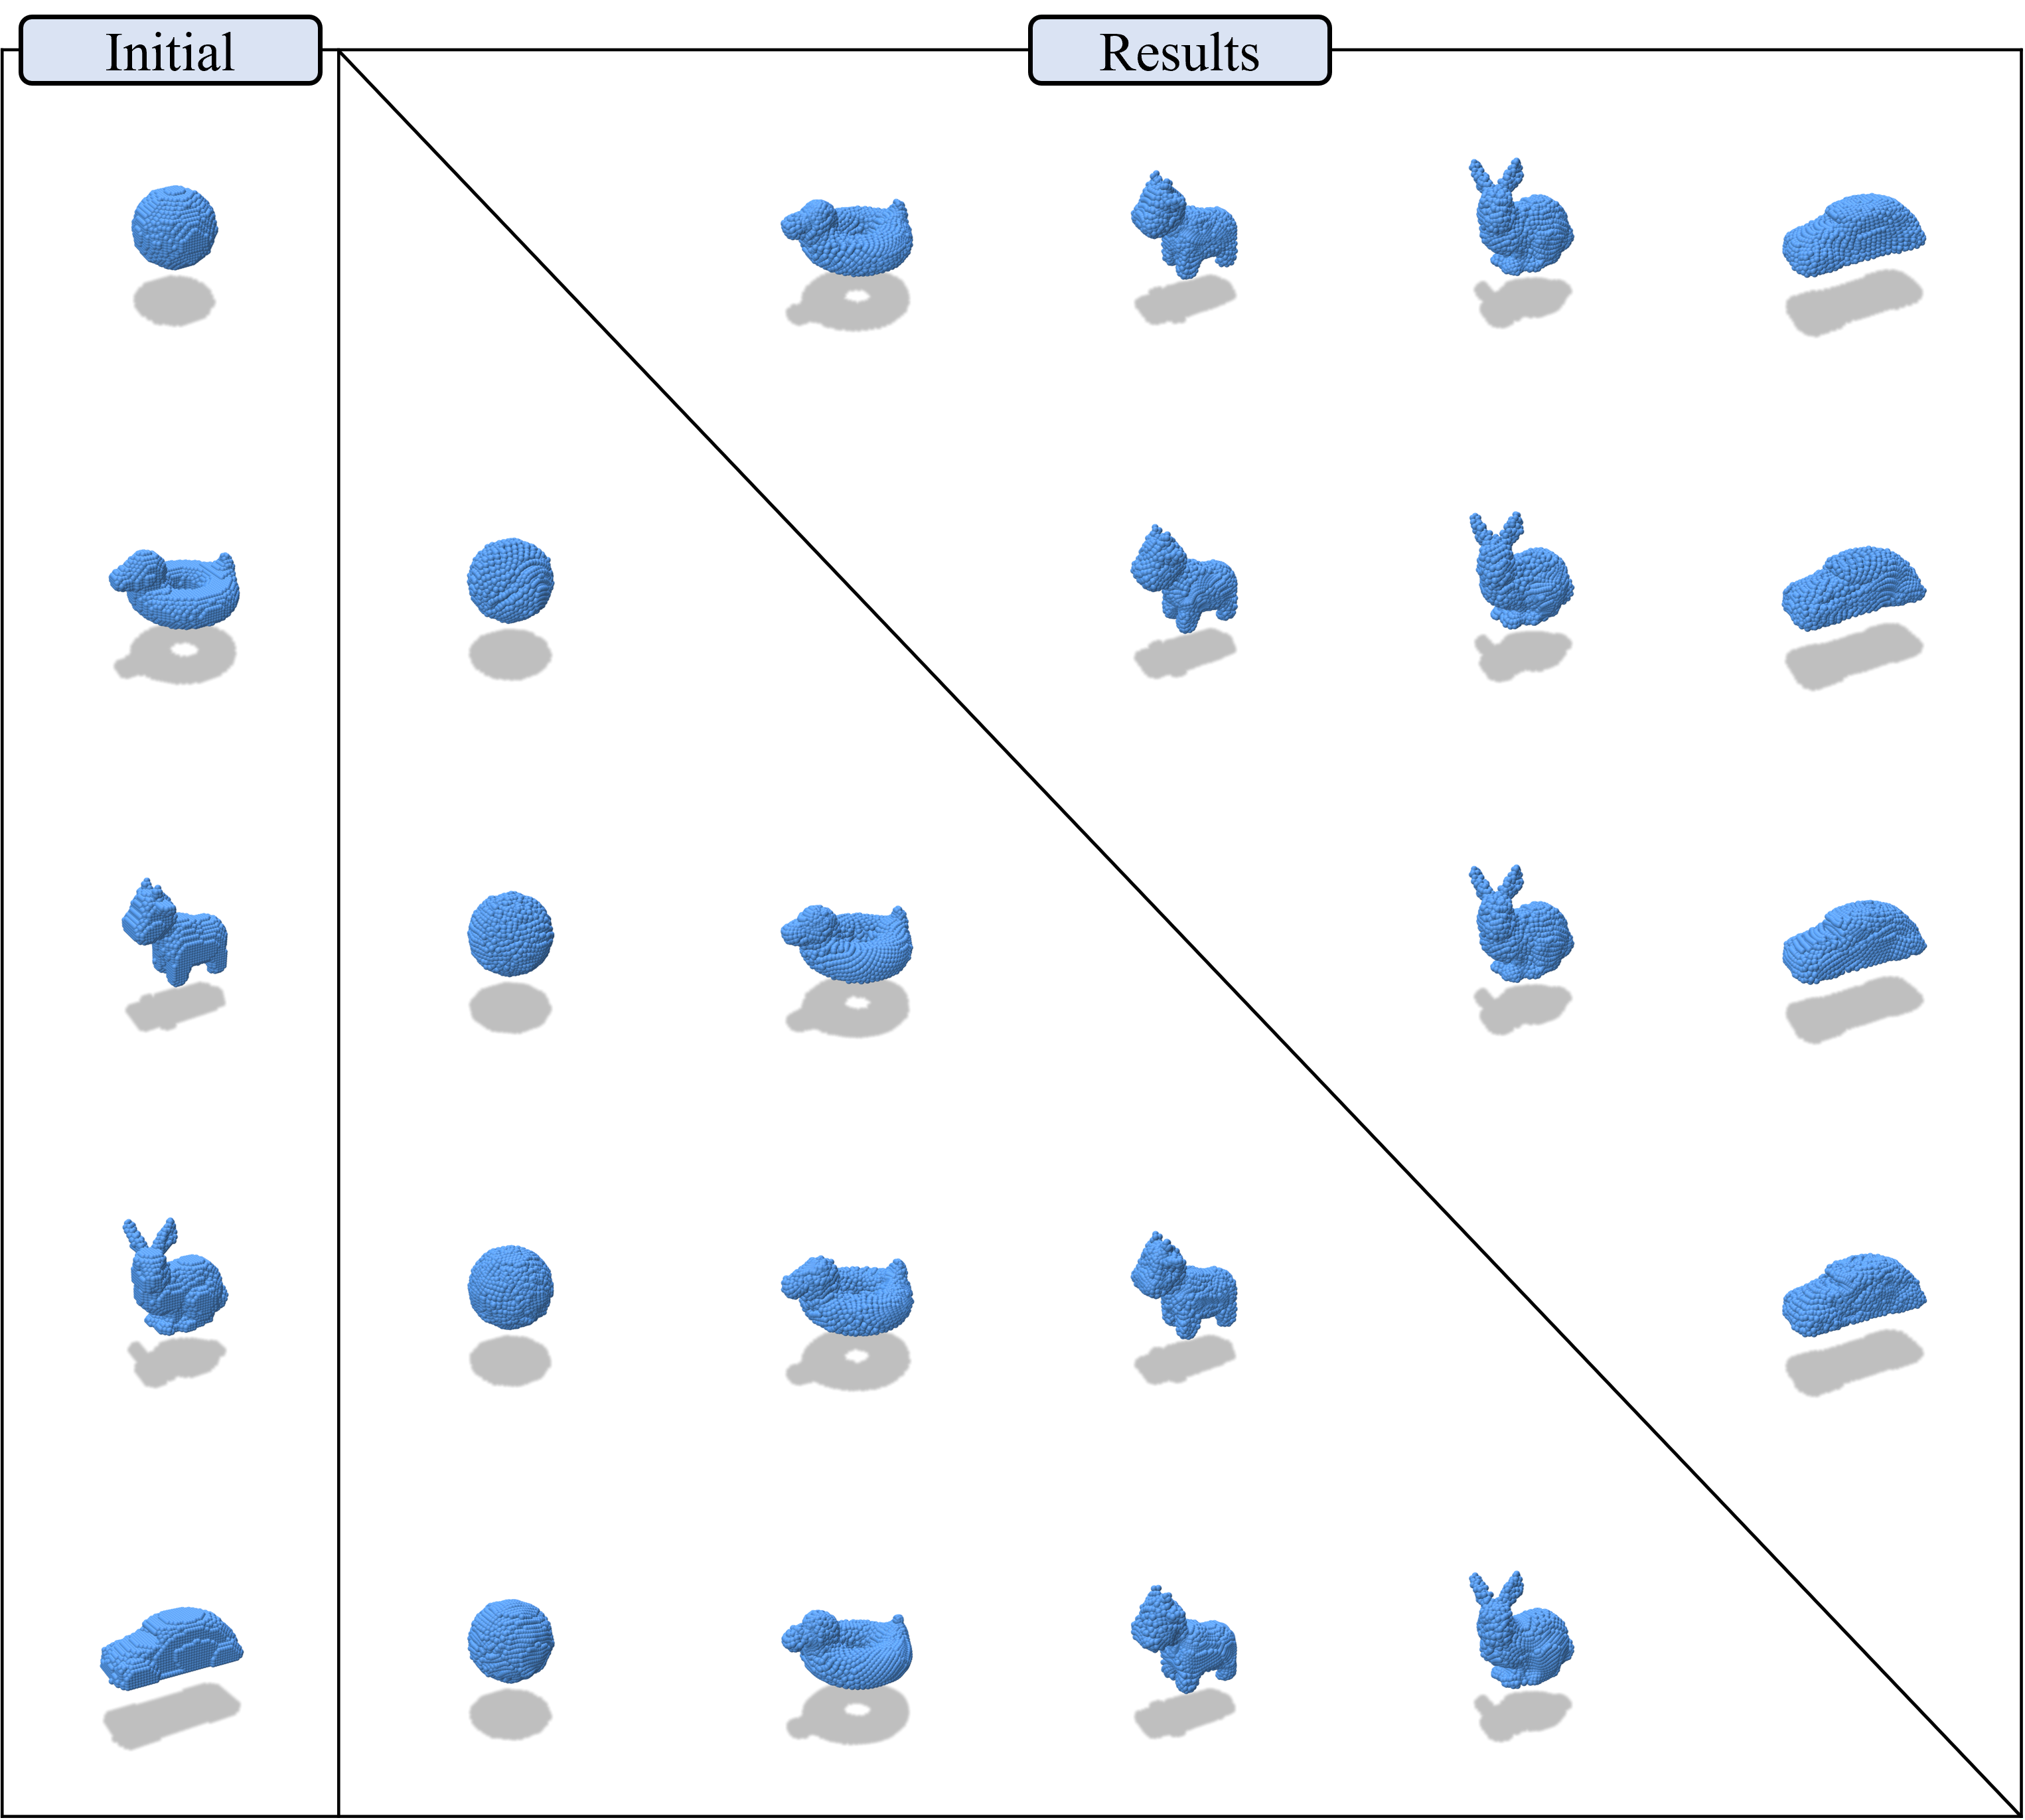
\includegraphics[width=\linewidth]{figs/Deform.png}
        \caption[{Pairwise shape morphing results among five distinct geometries}]{\textbf{Pairwise shape morphing results among five distinct geometries.} The left column shows the five initial meshes (sphere, duck/Bob, cow, bunny, and car); the grid on the right shows the resulting shapes for different targets. Self-morphs along the diagonal are omitted.}
        \label{fig:Overall_deform}
    \end{figure}
    
    \textbf{Smoothing Factor.}
    An additional element in achieving a high success rate was the application of a simple interpolation step during post-processing:
    \[
    \mathbf{F}^{n+1} \leftarrow (1 - \gamma)\,\mathbf{F}^{n+1} + \gamma\,\mathbf{F}^{n},
    \]
    where \(\gamma \in [0,1]\) is a smoothing factor.
    Larger \(\gamma\) values effectively suppress abrupt changes, leading to a smoother morph, whereas smaller \(\gamma\) values preserve faster convergence but may induce pronounced oscillations.
    In practice, we observed that setting \(\gamma\) beyond 0.5 made little difference visually, yet using \(\gamma = 1\) often prevented the morph from completing correctly.
    We primarily fine-tuned \(\gamma\) within the range of 0.95 to 0.98, striking a good balance between speed and stability.
    All specific \(\gamma\) values employed in our experiments are reported in Table~\ref{tab:params}.
    They were hand-tuned per example but were all generally set around 0.955. %—generally kept as small as possible to avoid excessive damping—while still ensuring visually coherent transformations.
    A more detailed demonstration of the the effects of varying \(\gamma\) (and its relative robustness above 0.5) can be found in our supplementary video.
    
    \textbf{Optimizer Comparisons.}
    We also performed a series of experiments to compare different optimizers, including Adam, Gradient Descent (GD), and the recently introduced Lion (Evolved Sign Momentum) \citep{chen2023symbolicdiscoveryoptimizationalgorithms}, highlighting the trade-off between convergence speed and stability.
    Figure~\ref{fig:Loss_comparison} shows loss curves for each optimizer.
    Adam consistently achieved lower loss in fewer iterations but exhibited significant oscillations near the optimum.
    In contrast, GD and Lion converged more steadily, though requiring more steps overall.
    By integrating the smoothing factor into Adam updates, we were able to retain much of Adam's fast convergence advantage while notably reducing the high-frequency vibrations in the morphing result.
    For a visual demonstration of how smoothing affects Adam's oscillations, we again refer to our supplementary video.
    
    \begin{figure}[ht!]
        \centering
        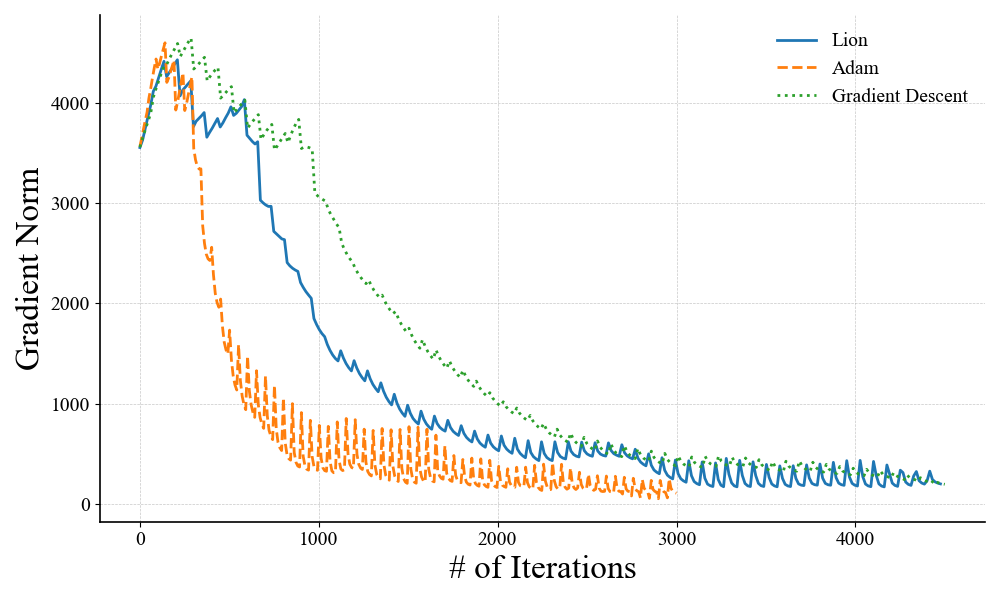
\includegraphics[width=0.7\linewidth]{figs/Loss_Comparision.png}
        \caption[{Comparison of loss curves under different optimizers (Adam, GD, Lion)}]{\textbf{Comparison of loss curves under different optimizers (Adam, GD, Lion) during the D to Dragon morphing task ($\beta_1 = 0.90$; learning rates: Lion/Adam = $1 \times 10^{-3}$, GD = 0.1).} Adam converges rapidly but suffers from strong oscillations near the optimum; GD and Lion converge more smoothly at a slower pace. Incorporating a smoothing factor ($\gamma$) into Adam's update reduces these oscillations, striking a balance between speed and stability.}
        \label{fig:Loss_comparison}
    \end{figure}



    \textit{Performance and parallelization.} Another benefit of our method is that the majority of our algorithm is parallelizable, due to our foundation on {MPM}. We produced a CPU-parallel implementation using OpenMP, leading to significantly shorter runtimes than a serial code.
 
    The performance of our parallel code on the various examples is reported in Table \ref{tab:performance}. 
    %offering a comprehensive overview of the time efficiencies realized through this methodology.
    We also demonstrate the strong scaling of our method in Figure \ref{fig:Core_per_time}; while our algorithm is not fully parallelizable and hence we do not expect perfect linear scaling, we still observe useful scaling from 1 to 24 cores (over 5x speedup). 

       \begin{figure}[ht!]
        \centering
        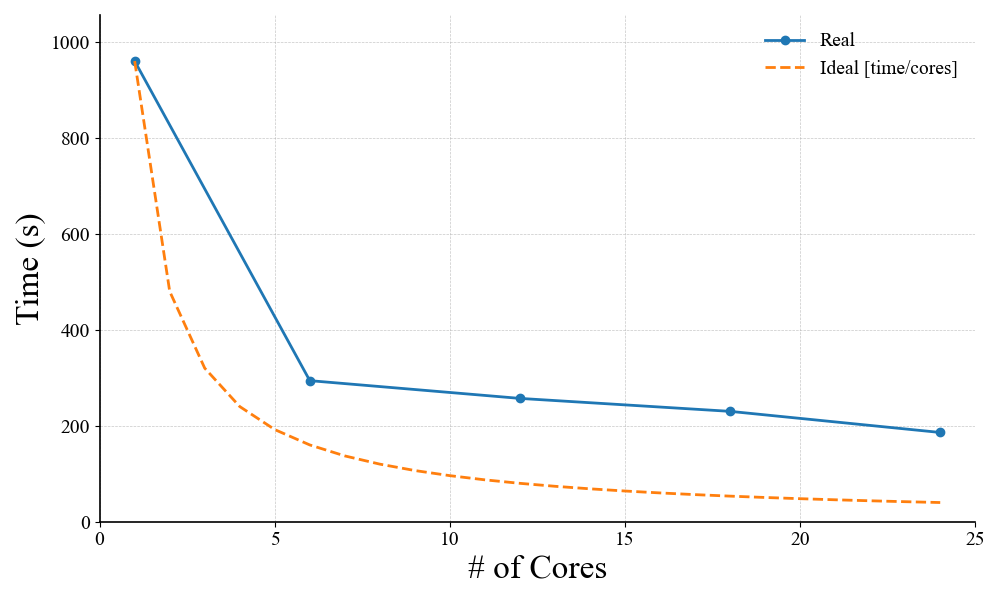
\includegraphics[width=0.7\linewidth]{figs/Plotting_Result.png}
        \caption[{Parallel scaling}]{\textbf{Parallel scaling.} As we run an example of our method with more cores (up to 24 cores), we observe nearly linear scaling.  The solid blue line indicates actual time, and theoretical time under perfect linear scaling is drawn with the yellow dashed curve.  Our method is not fully parallelized, so we do not expect linear scaling.}
        \label{fig:Core_per_time}
    \end{figure}

    \textit{Complex Object Animation.} In our complex object animation examples (see Figures \ref{fig:TVCG} and \ref{fig:Dragon}), we demonstrate that our approach can generate smooth morphing animations for complex surfaces and dynamic topology scenarios. In these examples, we test both letter models and a dragon model, which possess curves and topologies that could pose challenges for traditional shape morphing methods. The letter models showcase our method's ability to handle sharp edges and changing topologies, while the dragon model tests its capability to preserve intricate details during the morphing process.
    %Our approach successfully generates these animations .
    For the dragon model, we utilized a larger number of particles to better capture details throughout the morphing process (see Table \ref{tab:numofparticles}).
        
    We rendered these animations using the \textit{VDB from Particles} node in Houdini with a varying voxel size and applied ten iterations of Laplace smoothing to the resulting mesh on each frame for better visual fidelity.  
    Nonetheless, minor artifacts were observed in some of the letter models during the mesh generation process. These artifacts may be attributed to the complex topological transitions present in such models and could be mitigated in future work through enhanced interpolation methods or refined post-processing techniques.

    % We rendered this animation using the VDB from Particles node in Houdini with a varying voxel size and applied ten iterations of Laplace smoothing to the resulting mesh on each frame for better visual fidelity.

    
    %We also applied two iterations of Laplace smoothing to the mesh generated from our particles on each frame.
    
    %During the rendering process, we implemented an additional refinement step to enhance the visual quality of the final result. This step involved a remeshing process, which was crucial for achieving a cleaner and more polished representation of the objects. The remeshing helped to smooth out any irregularities in the particle distribution and create a more uniform surface, particularly important for complex models like the dragon. This process allowed us to achieve a smoother, more refined, and visually appealing final result that accurately represents the intended morphed shapes while maintaining the integrity of the original models' features.

     \begin{figure}[!bt]
        \centering
        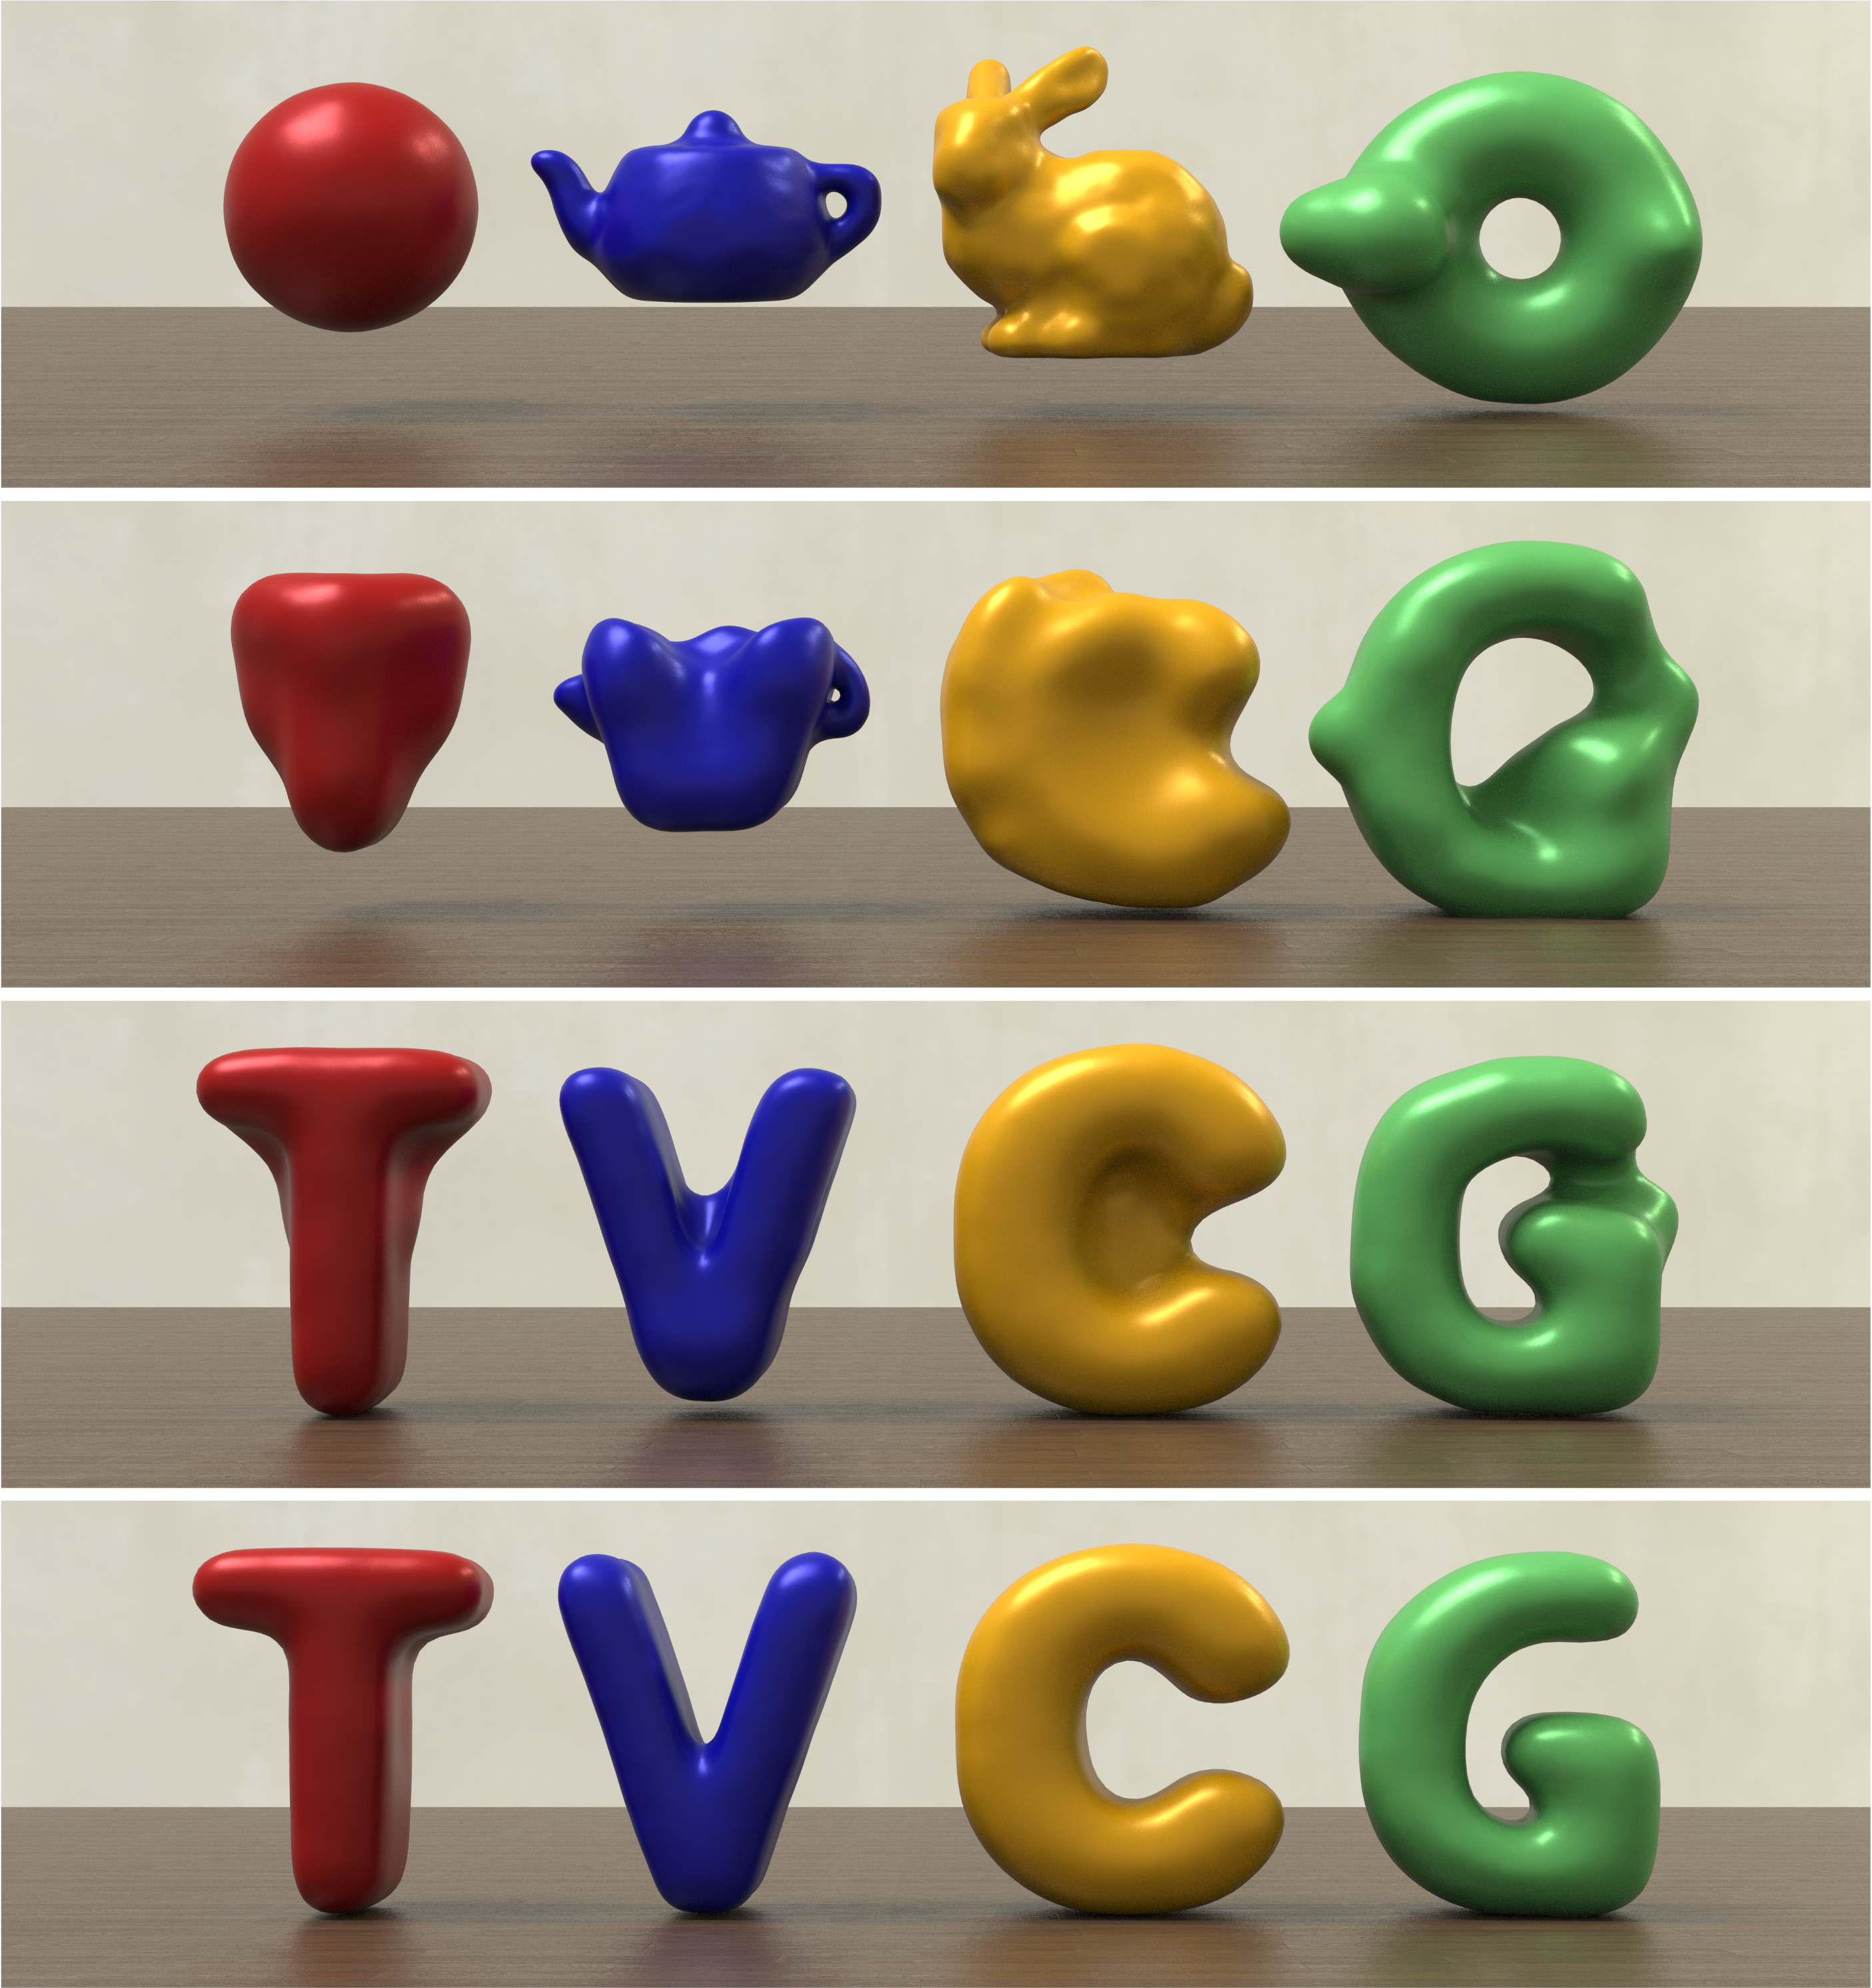
\includegraphics[width=\linewidth]{figs/TVCG_figure.png}
        \caption[{Morphing example with letters}]{\textbf{Morphing example with letters.} This example demonstrates the capability of our morphing technique to capture topological changes and fine details during a morph. The sequence maintains accurate detail as each form transitions into the next, showing the potential for making practical animations with our method.}
        \label{fig:TVCG}
    \end{figure}

     \begin{figure}[!bt]
        \centering
        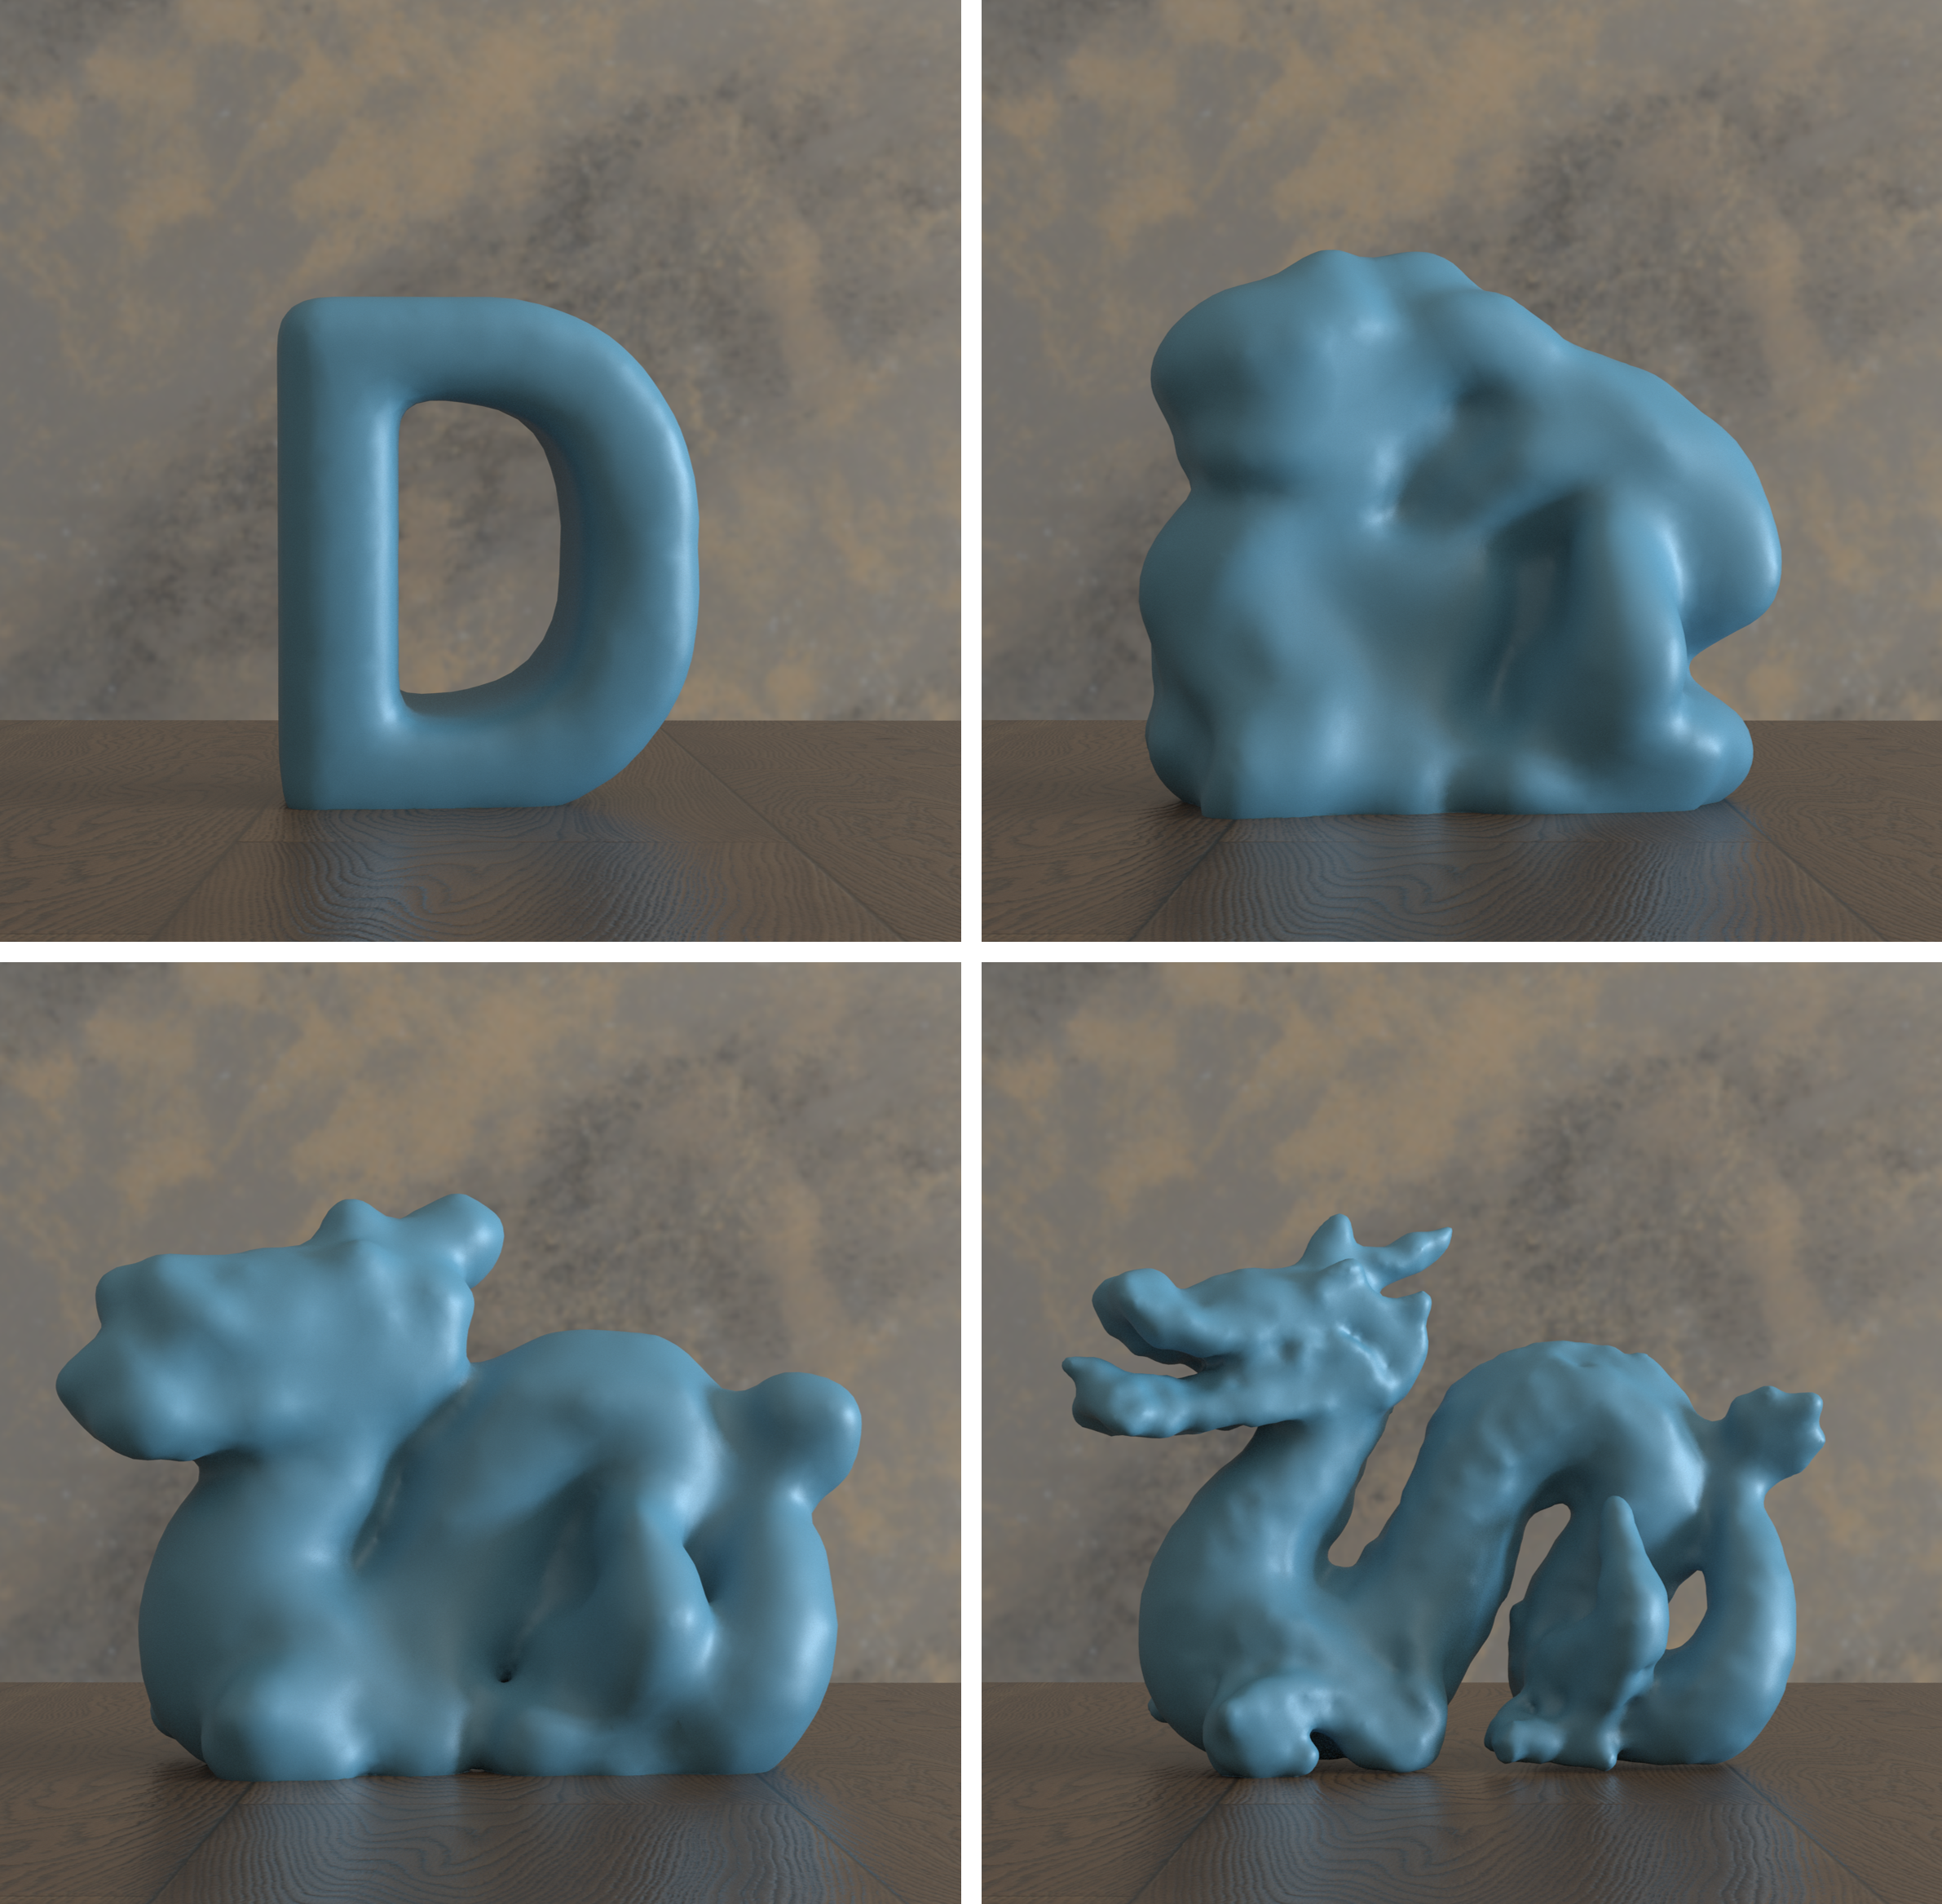
\includegraphics[width=\linewidth]{figs/dragon_v2.png}
        \caption[{Morphing dragon example}]{\textbf{Morphing dragon example.} This example demonstrates the transformation from the letter `D' into a dragon model. Our method effectively handles the complex topology changes that occur during the morph, preserving both surface details and structural coherence.}
        \label{fig:Dragon}
    \end{figure}

    \begin{table}[!bt]
      \centering
      \caption[{Number of particles for our complex examples}]{\textbf{Number of particles for our complex examples.}}
      \begin{tabular}{lccc}
        \toprule
        \textbf{Example} & \textbf{\# of Timesteps} & \textbf{Target \# of Particles} & \textbf{Initial \# of Particles} \\ 
        \midrule
        Sphere to T    & 840  & $1.99 \times 10^4$  & $3.76 \times 10^4$ \\ 
        Teapot to V    & 840  & $ 2.48 \times 10^4$  & $2.98 \times 10^4$ \\
        Bunny to C     & 840  & $3.14 \times 10^4$  & $1.75 \times 10^4$ \\
        Bob to G      & 840 & $1.25 \times 10^4$  & $1.75 \times 10^4$ \\
        D to Dragon    & 950 & $3.92 \times 10^4$  & $2.46 \times 10^4$ \\
        \bottomrule
      \end{tabular}
      \vspace{1mm}
      \label{tab:numofparticles}
    \end{table}

    \textit{Morphing Under Physical Disturbances.}
    \label{sec:physical-disturbance}
    \begingroup
    To evaluate the physical robustness of our MPM-based morphing framework, we designed and conducted experiments under various disturbance conditions. These experiments go beyond static shape matching and assess system stability under external forces and material variability, reflecting more realistic physical environments.
    
    \textbf{Gravity-induced deformation.}  
    A constant vertical gravitational force of $3.5\,\mathrm{m/s^2}$ was applied throughout the morphing process.  
    This force induced elastic sagging in the lower portion of the object, replicating stress experienced by real-world structures under load.  
    The object exhibited realistic deformation while gradually converging toward the target shape, maintaining its elastic properties throughout (see top of Figure~\ref{fig:external_disturbances}).

    \begin{figure}[ht!]
        \centering
        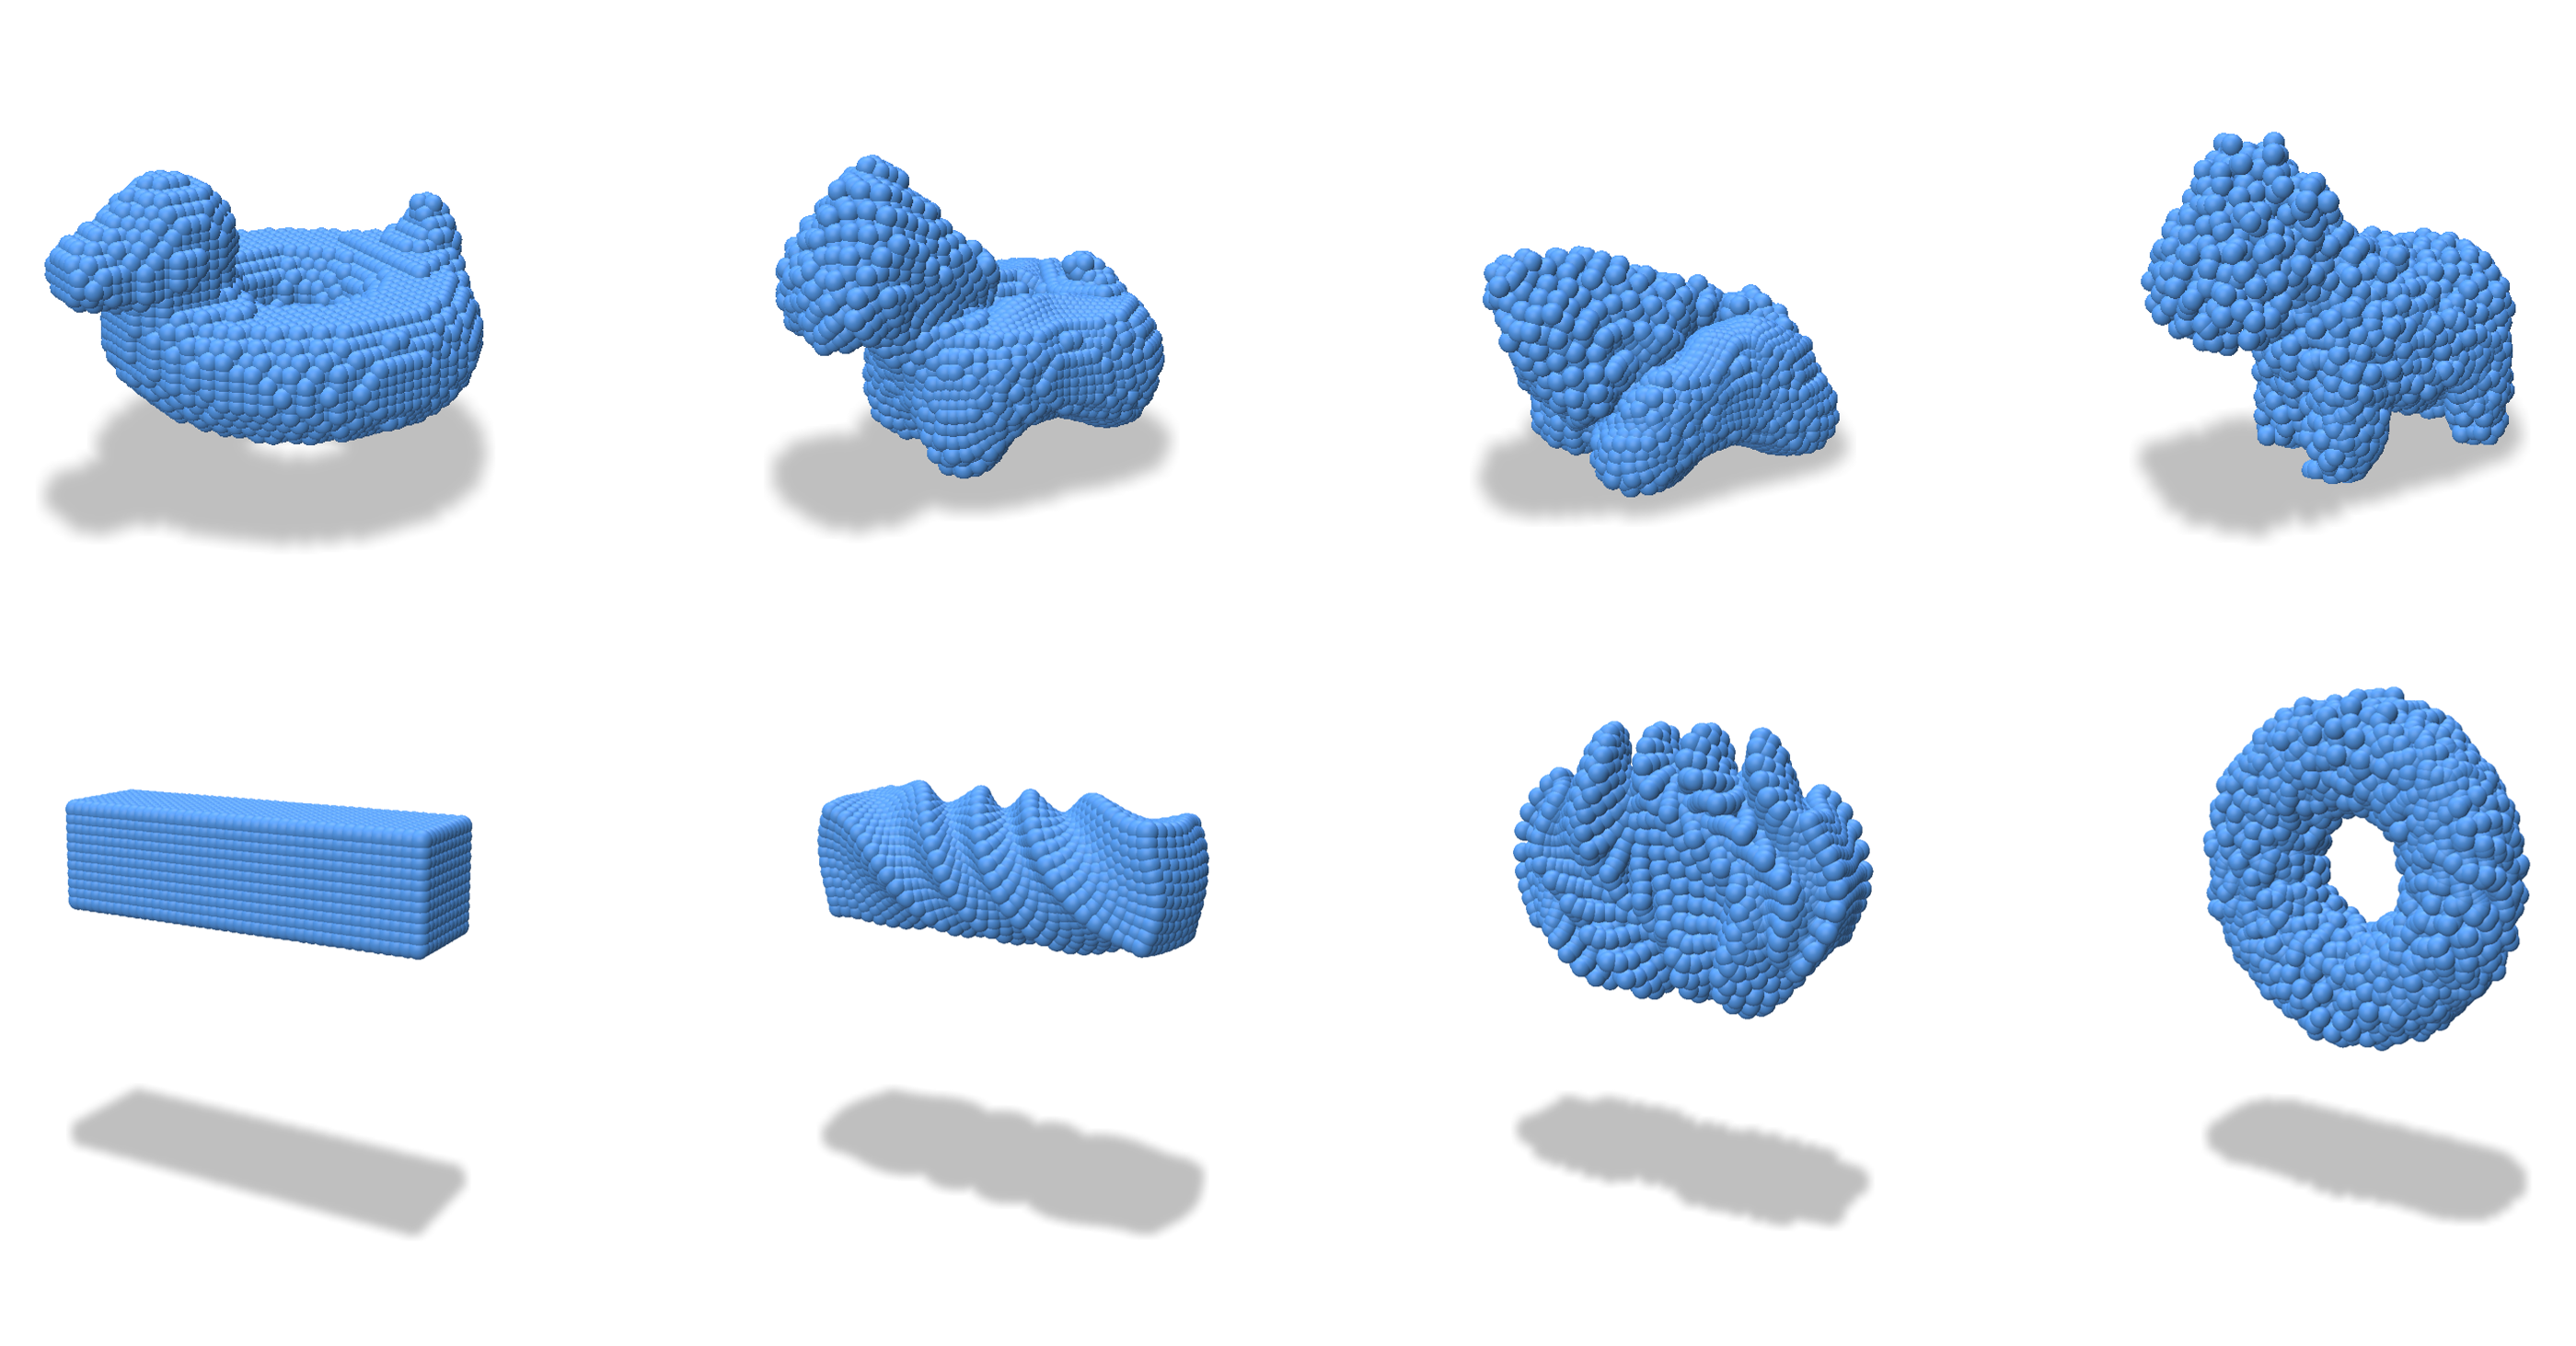
\includegraphics[width=0.8\linewidth]{figs/external_force_disturbance.png}
        \caption[{Morphing under physical external forces}]{\textbf{Morphing under physical external forces.} \textbf{Top:} Under a constant vertical gravitational force of $3.5\,\mathrm{m/s^2}$, 
            the object experiences elastic sagging yet steadily converges to the target shape.
            \textbf{Bottom:} When torque is applied to one end while fixing the other,
            the object undergoes twist deformation, but the method robustly handles the stress and completes the morph.}
        \label{fig:external_disturbances}
    \end{figure}
    
    \textbf{Twist-induced stress.}  
    One end of the object was fixed while a torque was applied to the other end, resulting in a non-uniform stress field.  
    Strong twisting occurred near the center of rotation during the initial steps, but the system successfully absorbed the stress and progressed toward the target.  
    The final configuration preserved a physically plausible twist while completing the morph (see bottom of Figure~\ref{fig:external_disturbances}).
    
    \textbf{Material stiffness variation.}  
    We varied the Young’s modulus $E$ from $2.5 \times 10^4$ to $1.0 \times 10^5$, with the Poisson’s ratio $\nu$ fixed at 0.3.  
    In both free morphing and vertical compression scenarios, lower stiffness values produced larger deformations and slower convergence, while higher stiffness led to more rigid responses and faster convergence. Nonetheless, all cases ultimately closely reached the target shape.
    
    These results demonstrate that our MPM-based differentiable simulation can handle physically realistic disturbances, including external forces and material variations, without introducing instability or failing to reach the target shape.  
    % While geometric morphing methods may perform well in idealized or purely interpolative settings, they may lack the capacity to respond effectively to such physical disturbances.  
    % By directly modeling these interactions through its constitutive formulation, our approach offers a practical advantage in scenarios where physical consistency is important.
    \endgroup
    
    \begin{figure}[ht!]
        \centering
        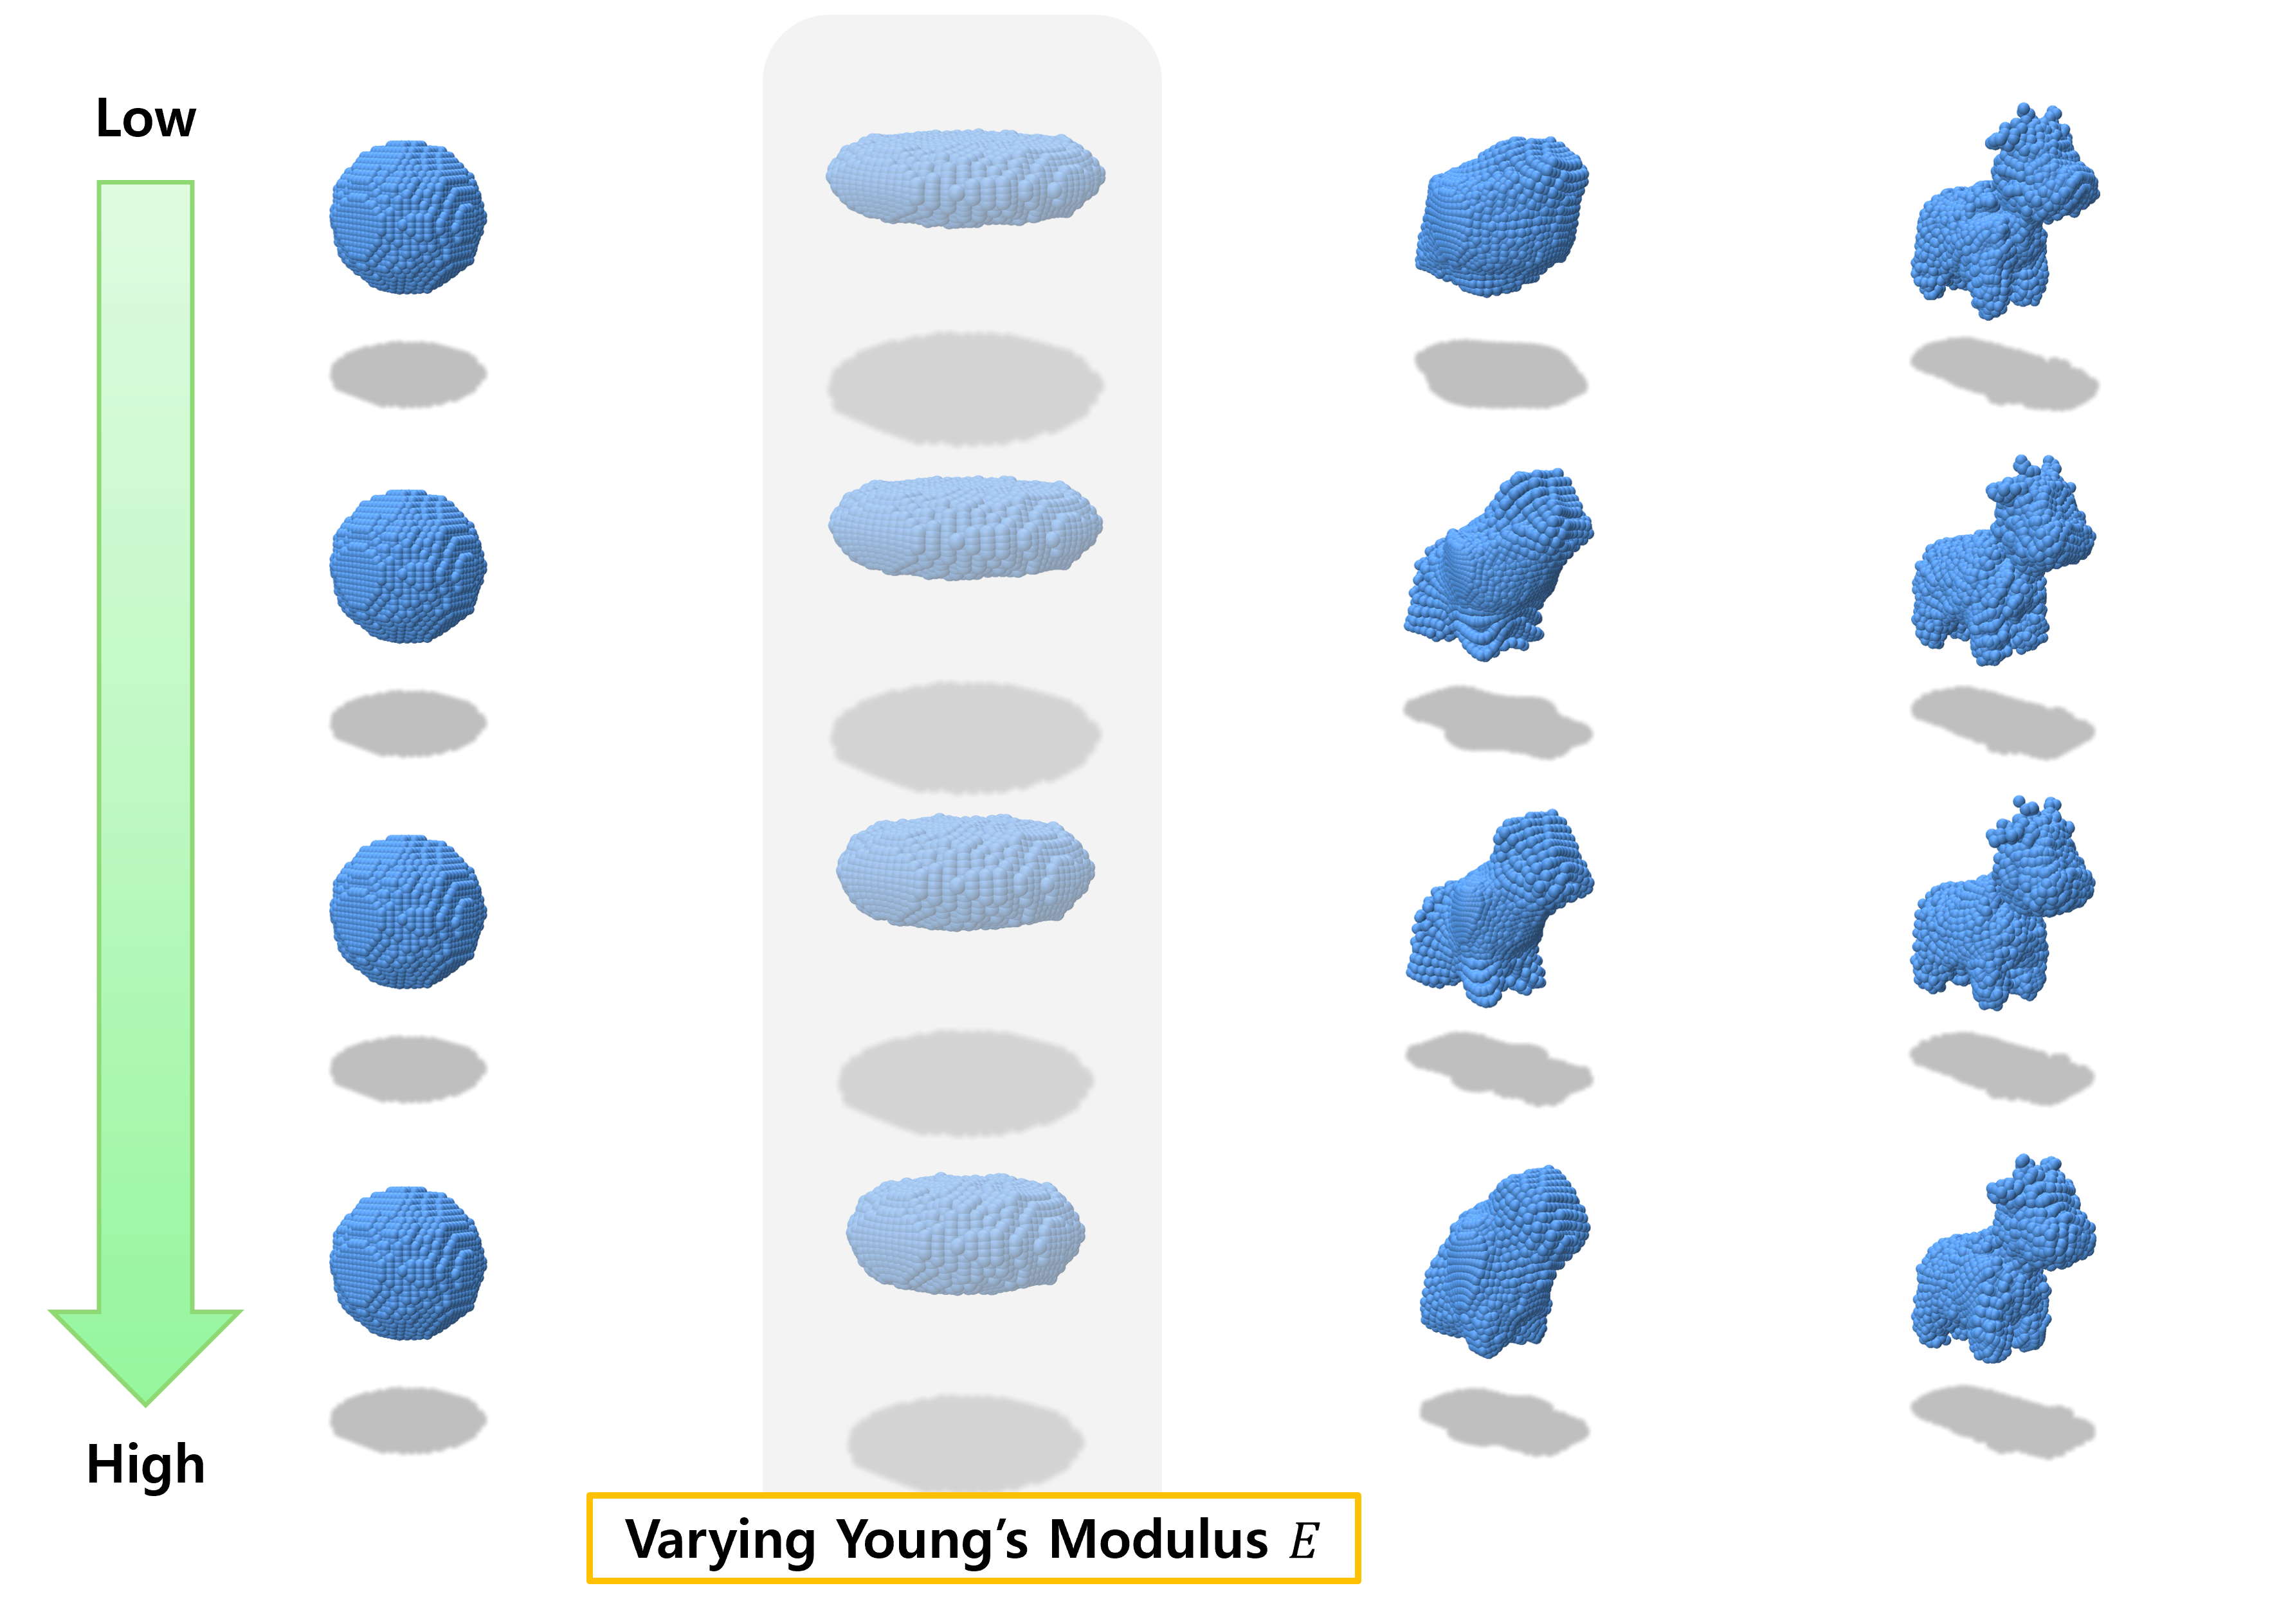
\includegraphics[width=0.8\linewidth]{figs/material_difference.png}
        \caption[{Morphing behavior under vertical compression across varying material stiffness}]{\textbf{Morphing behavior under vertical compression across varying material stiffness.} The highlighted middle column illustrates the deformation differences observed for varying Young’s modulus values ($E = 2.5 \times 10^4$ to $1.0 \times 10^5$, with $\nu = 0.3$ fixed). Softer materials undergo more pronounced compression, while stiffer materials retain their shape better and tend to converge more quickly to the target configuration.}
        \label{fig:material_difference}
    \end{figure}

\section{Chapter Summary}
\label{sec:shape_morph_summary}
    This chapter presented a physics-based shape morphing framework built upon differentiable Moving Least Squares Material Point Method (MLS-MPM). Rather than prescribing particle trajectories or applying manually designed external forces, our approach directly controls internal deformation through optimized per-particle control deformation gradients. By differentiating through the simulation and optimizing these controls, the framework enables target-driven shape transformations while retaining the underlying material dynamics.
    
    To improve optimization stability, we introduced a log-based nodal mass loss function with an additional penalty term,
    which mitigates mass ejection artifacts without requiring explicit point-to-point correspondences between source and
    target geometries. We further employed gradient-based optimization with Adam, multiple optimization passes, and
    chained simulation networks to support complex and long-duration morphing sequences.
    
    Through a variety of morphing experiments, we demonstrated the ability of our framework to handle substantial geometric
    deformations, topology changes, and fine-scale shape features. Additional experiments involving gravitational forces,
    twisting, and variations in material stiffness demonstrated the flexibility of deformation-gradient-based control under
    different physical conditions. Together, these results establish differentiable MLS-MPM as a practical foundation
    for directing deformable-object animations through physics-based optimization.
    